%!TEX root = ../../super_main.tex

\section{Participant Interaction}
\label{sec:participant_interaction}
Limited screen real estate characterizes user interfaces for mobile systems and is a general concern when designing user interfaces for these, compared to designing GUIs for desktop systems \parencite[cha. 21]{mobile_computing_constraints}. The limited screen real estate is generally solved by more navigation and by having more focus on a few visible elements at a time. We have therefore split our graphical user interface into a few logical screens with different views and implemented navigation between them in order to improve the interaction. Having all functionality on one screen tends to be less portable to many different screen sizes and cause overlapping hit areas for buttons and other interactive elements.
\\\\
During the construction of the participant interface we have followed the Google Material Design\footnote{https://www.google.com/design/spec/material-design/} manual, which is a design manual provided by Google for the Android platform. This design manual helps designing an interface using good design practices on the Android platform. By adhering to this design manual, we hope to achieve a user friendly interface for participants that fits as many different users as possible. This will guide us in improving different aspects of our application, such as utilization of screen estate and usability in general without having to design an interface from the ground up. Throughout this section we provide mockups together with descriptions of the implementation of the user interface on the mobile device.

\subsection{Opening the Application}
\label{sub:opening_the_application}
When a participant opens the mobile application, the participant is presented with an initial screen, as seen in \figref{fig:initial_screen}. The idea with this screen is to welcome the participant to the application. Currently, it does not supply the participant with any information, but one could imagine that this view would, in a potential future release, provide the participant with usable information, such as progress in the current campaign, clarification of what concepts and principals the participant must know. This screen could possibly also contain some motivational factor, provided by the customers, e.g. a ``prize'' for participation.

% Initial screen
\begin{figure}[!htbp]
    \begin{subfigure}[!t]{.48\textwidth}
        \centering
        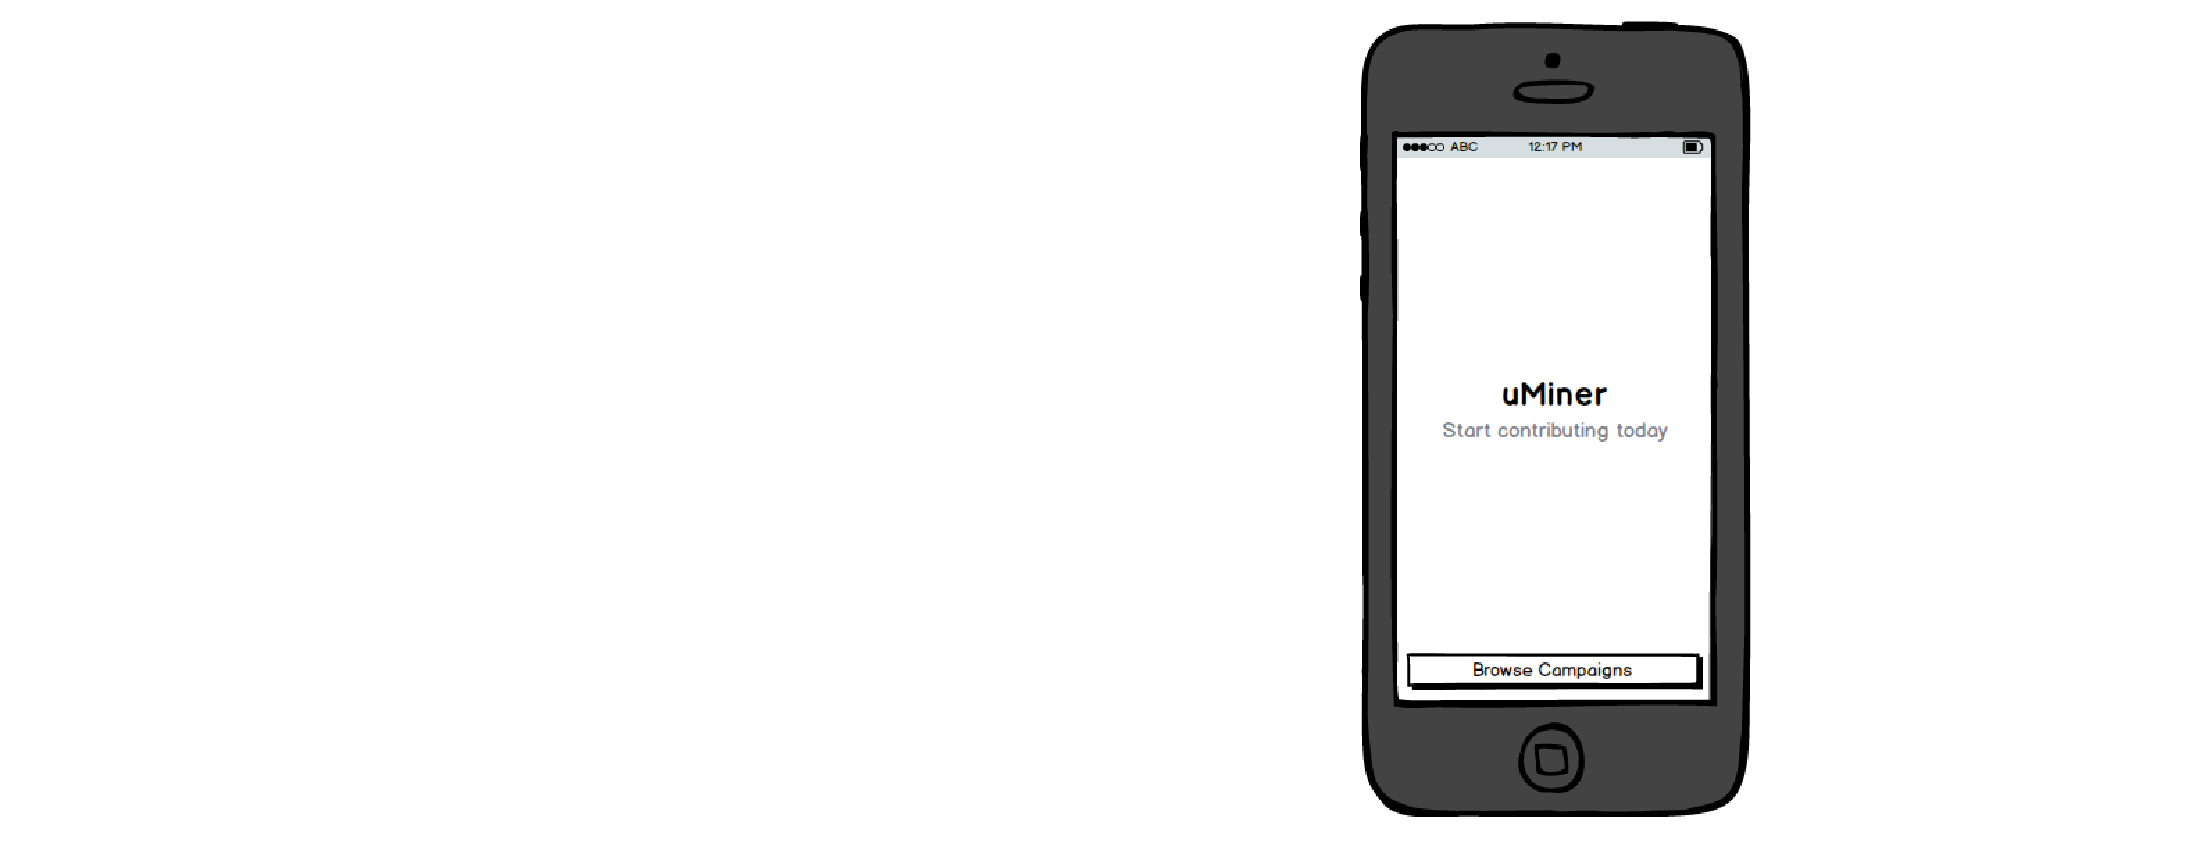
\includegraphics[width=.7\linewidth]{mockups/homepage}
        \caption{Mockup of the initial screen.}
        \label{fig:mockup_initial_screen}
    \end{subfigure}%
    \begin{subfigure}[!t]{.52\textwidth}
    \centering
        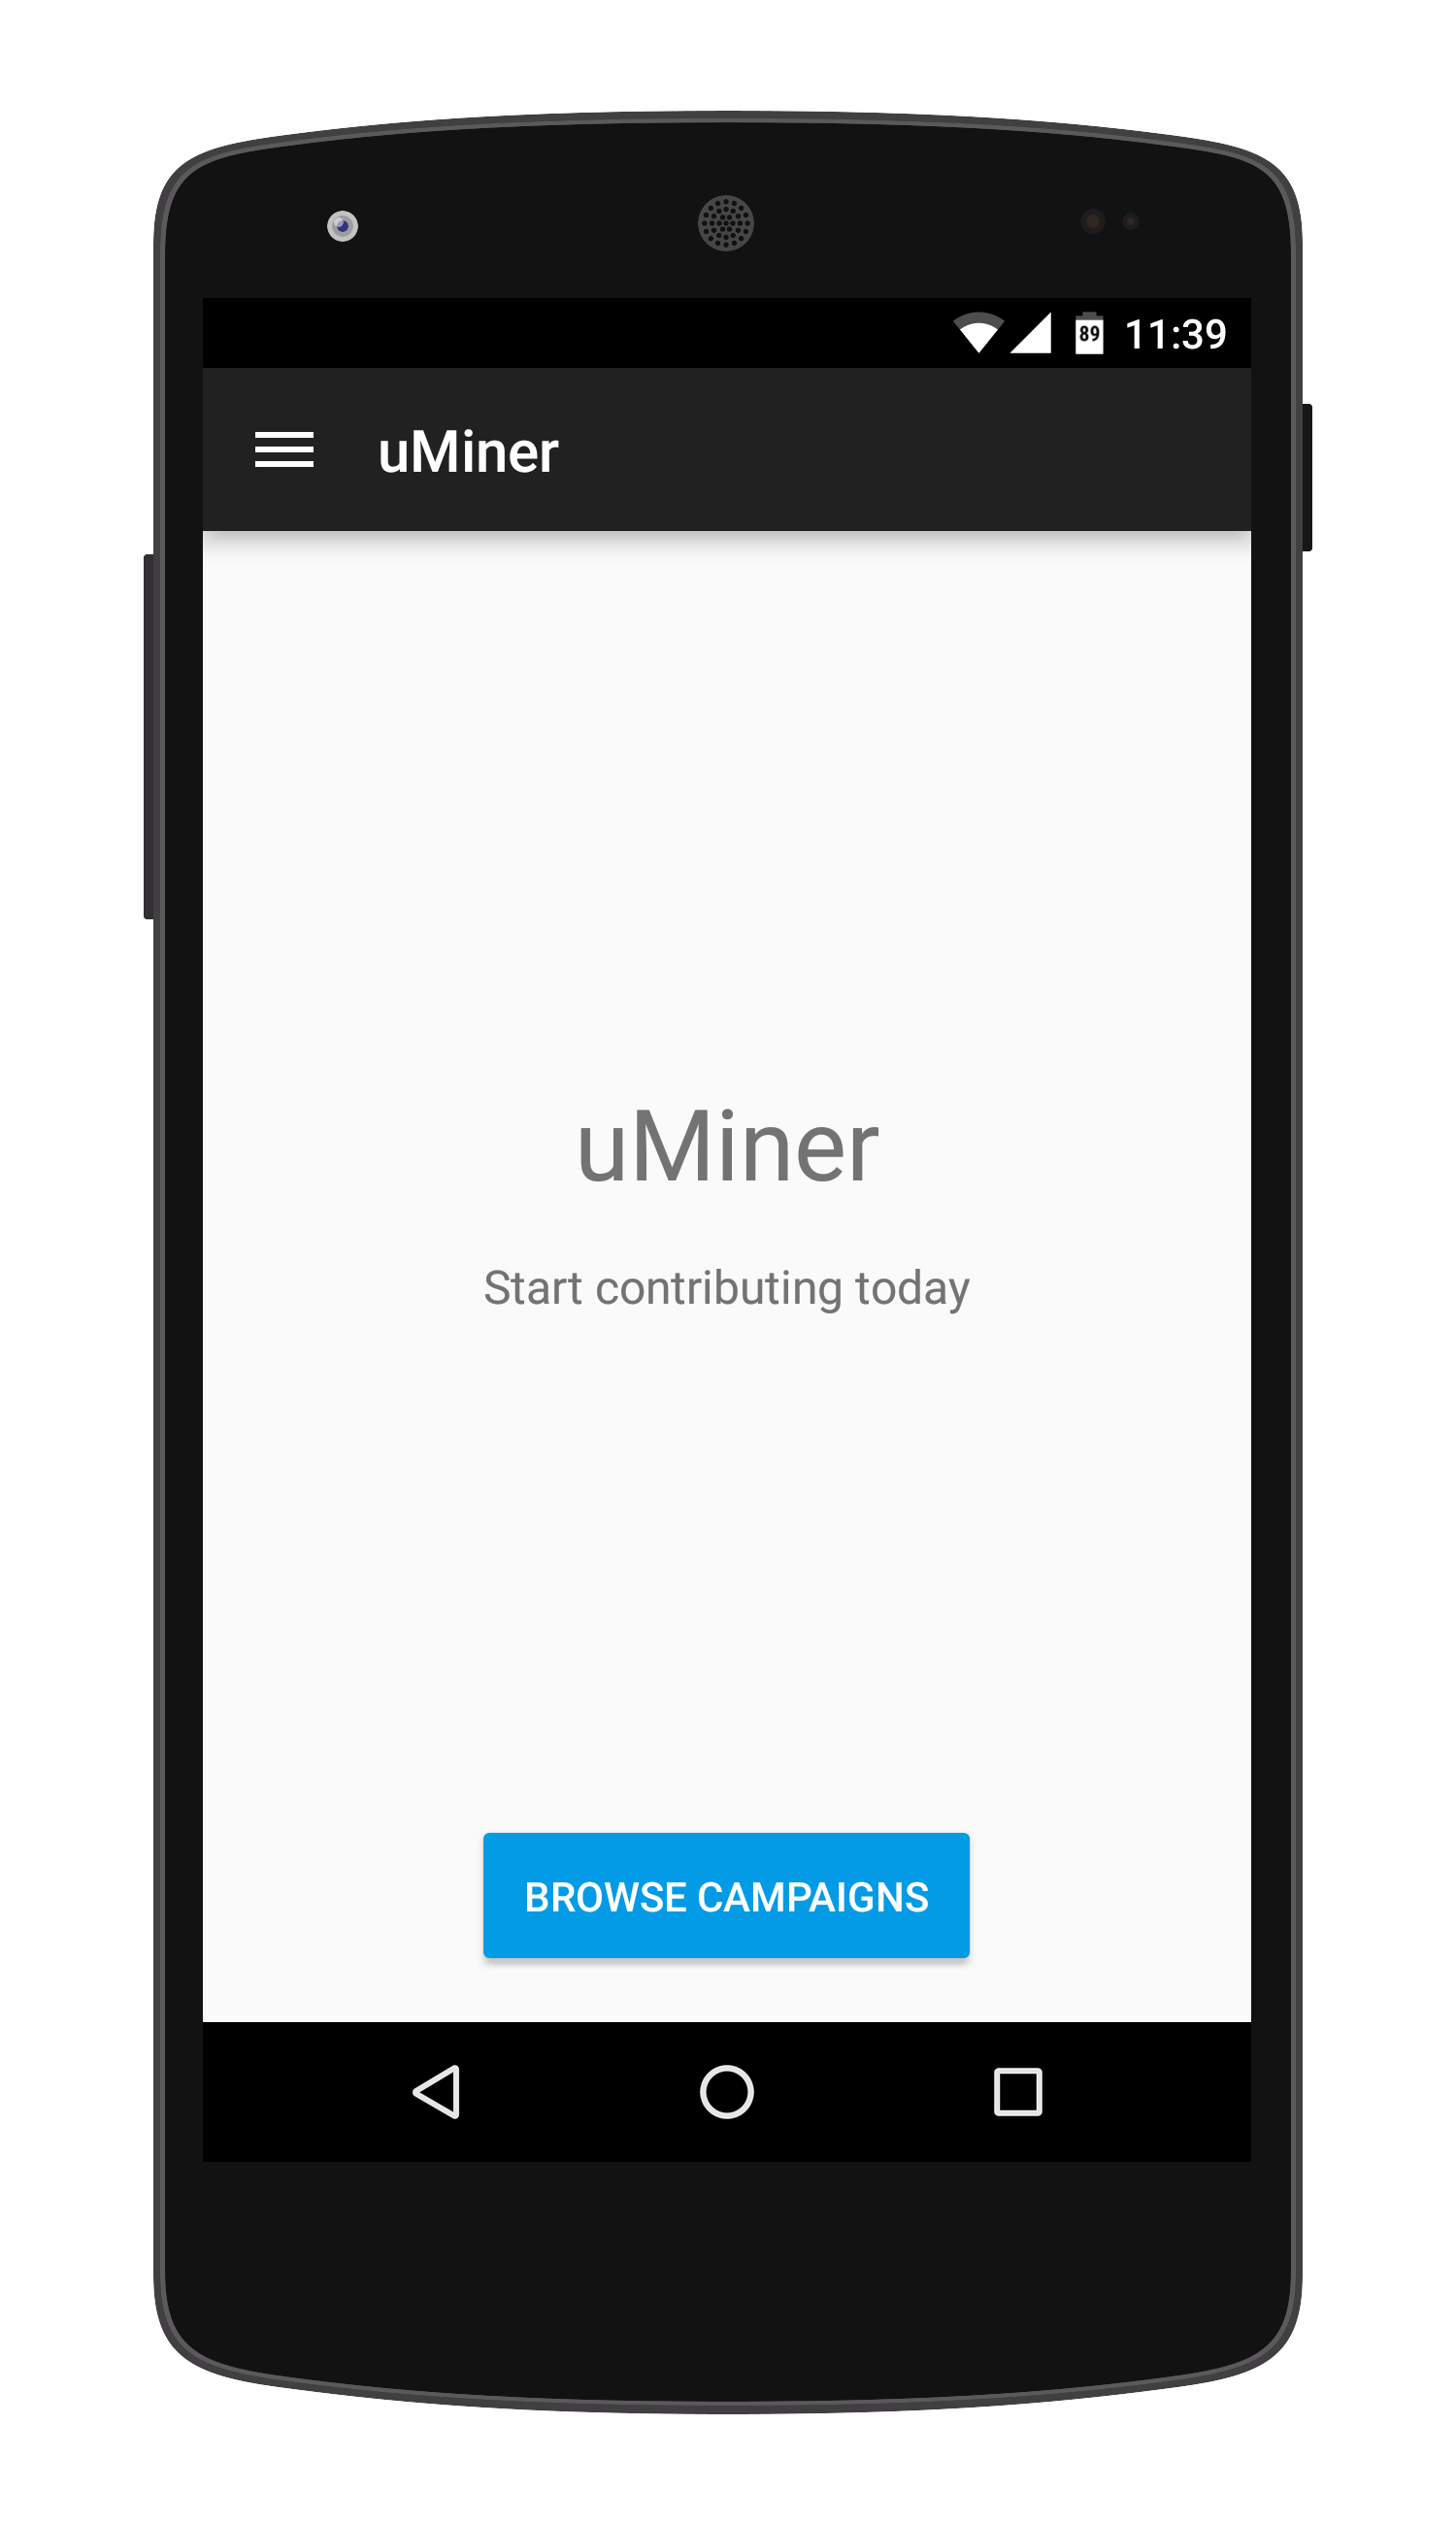
\includegraphics[width=.73\linewidth]{user_interfaces/client/client_uminer_home_with_phone}
        \caption{Implementation of the initial screen.}
        \label{fig:implementation_initial_screen}
    \end{subfigure}
    \caption{Mockup and implementation of the initial screen of the application.}
    \label{fig:initial_screen}
\end{figure}
\FloatBarrier

The participants must either use the drawer menu displayed in \figref{fig:navigation} or press the \emph{browse campaigns}-button in the initial view to navigate to other views in the application. The navigation menu contains three elements, namely ``Browse campaigns'', ``Join specific'', and ``Current campaign'', which each takes the participant to different parts of the application. This menu will at all times be available in the primary application by swiping from the left edge of the screen, or by pressing the hamburger icon ($\equiv$) next to the uMiner title in the top bar. 

\begin{description}
    \item[``Browse campaigns''] redirects the participant to a view containing brief information about all of the publicly available campaigns, as seen in \figref{fig:public_campaigns}.

    \item[``Join specific''] redirects the participant to a view, as seen in \figref{fig:specific_campaign}, where it is possible to search for a specific campaign by providing a campaign identifier.

    \item[``Current campaign''] redirects the participant to a campaign specification view, as seen in \figref{fig:leave_campaign_no_dialog}, displaying more information about the campaign that they are currently contributing to. If the participant have not yet joined a campaign, a message will briefly be displayed on the screen, informing the participant about this.
\end{description}

% Navigation
\begin{figure}[!htbp]
    \centering
    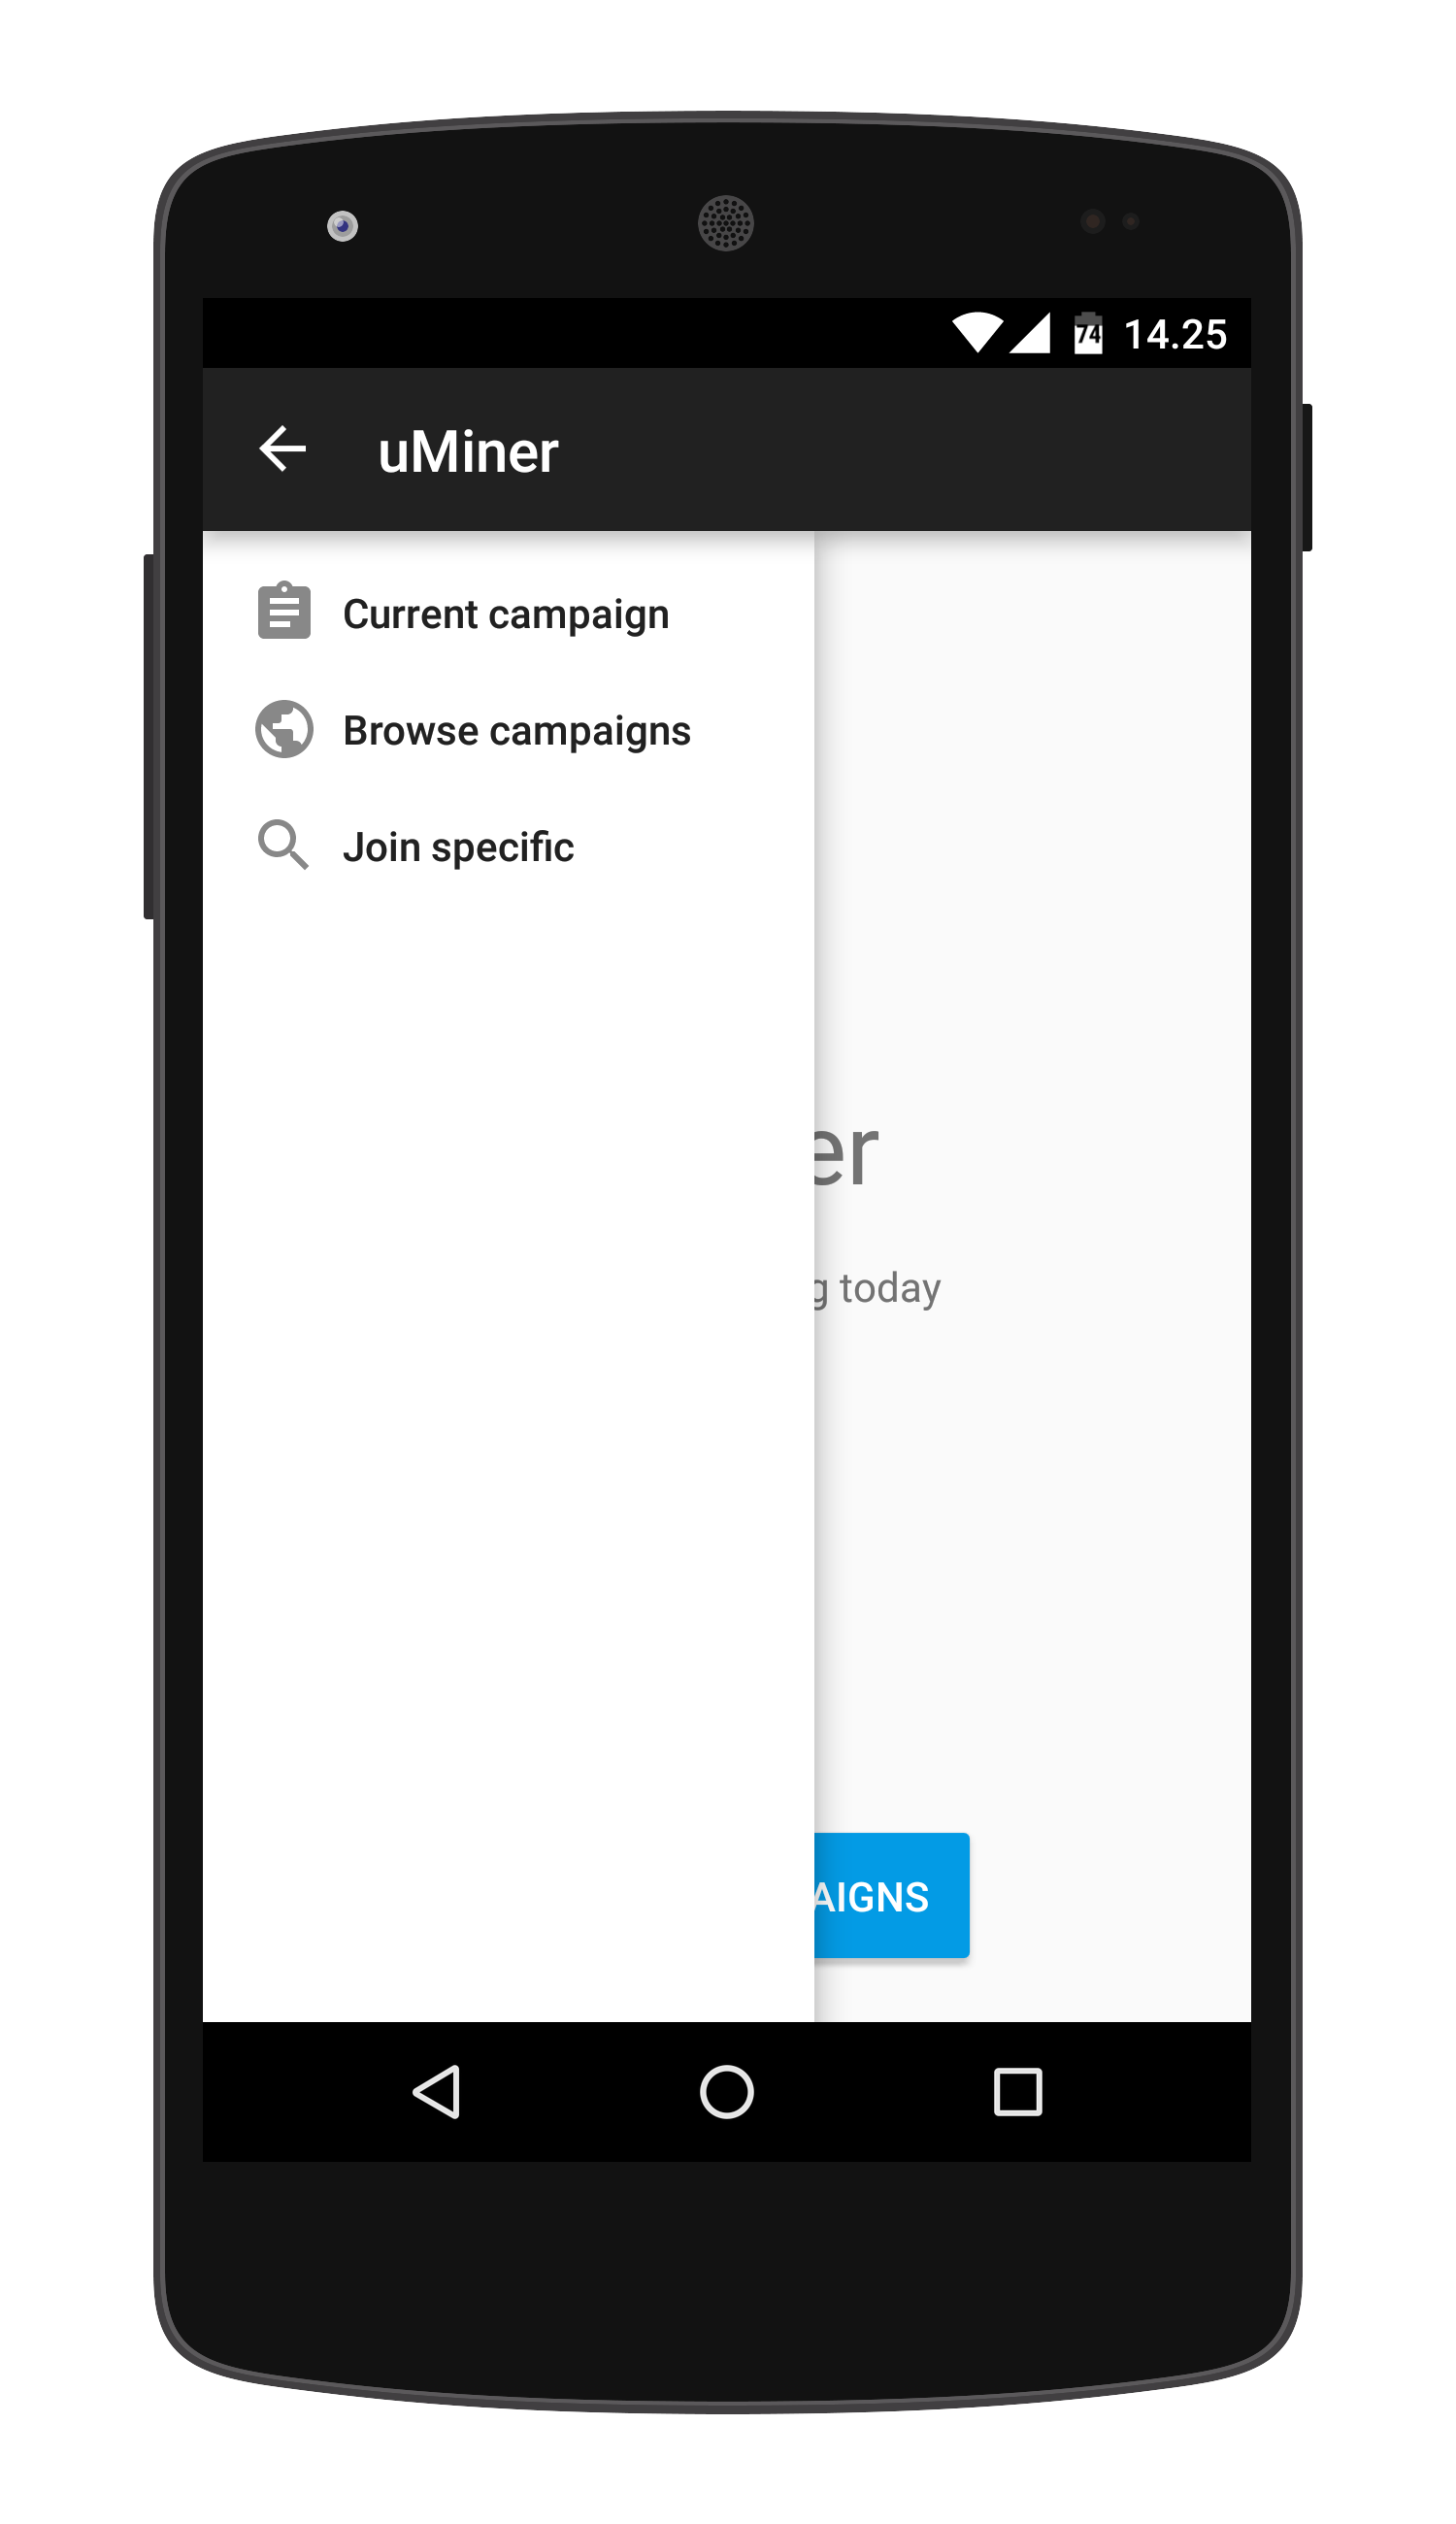
\includegraphics[width=.35\linewidth]{user_interfaces/client/client_drawer_menu_with_phone}
    \caption{Navigation through the application.}
    \label{fig:navigation}
\end{figure}
\FloatBarrier

\subsection{Browsing Campaigns}
\label{sub:browsing_campaigns}



 If participants want to contribute to a campaign, they may browse the publicly available campaigns, which can be done through the screen seen in \figref{fig:public_campaigns}. All the publicly available campaigns are listed here, each with its own entry displaying the title alongside the author of the campaign. If the participant wishes to learn more about one of the listed campaigns, he can press on that campaign and be redirected to a view similar to the one seen in \figref{fig:campaign_specification}, where more detailed information about the selected campaign is shown. 
\\\\
We have for the implementation of the listing of campaigns utilized a design pattern called the \emph{view holder} design pattern \parencite{view_holder_pattern} together with an Android \mono{Adapter}. The \mono{Adapter} makes sure that we can reuse \mono{View} instances and thus prevents constant allocation and deallocation of \mono{View}s when the user is scrolling the list. Using the heap excessively is expensive in terms of CPU cycles in Java and triggers the garbage collector to run more than necessary \parencite{android_garbage_collection}. We would thus like to minimize use of the heap. Reusing \mono{View}s helps reduce battery consumption and should improve the general performance perceived by users and prevent stuttering in the graphical interface. Alongside the \emph{view holder} pattern, only the data, which is strictly necessary for displaying the list is downloaded for this screen. More detailed information is fetched when needed by other screens.

% Publicly available campaigns
\begin{figure}[!htbp]
    \begin{subfigure}[!t]{.48\textwidth}
        \centering
        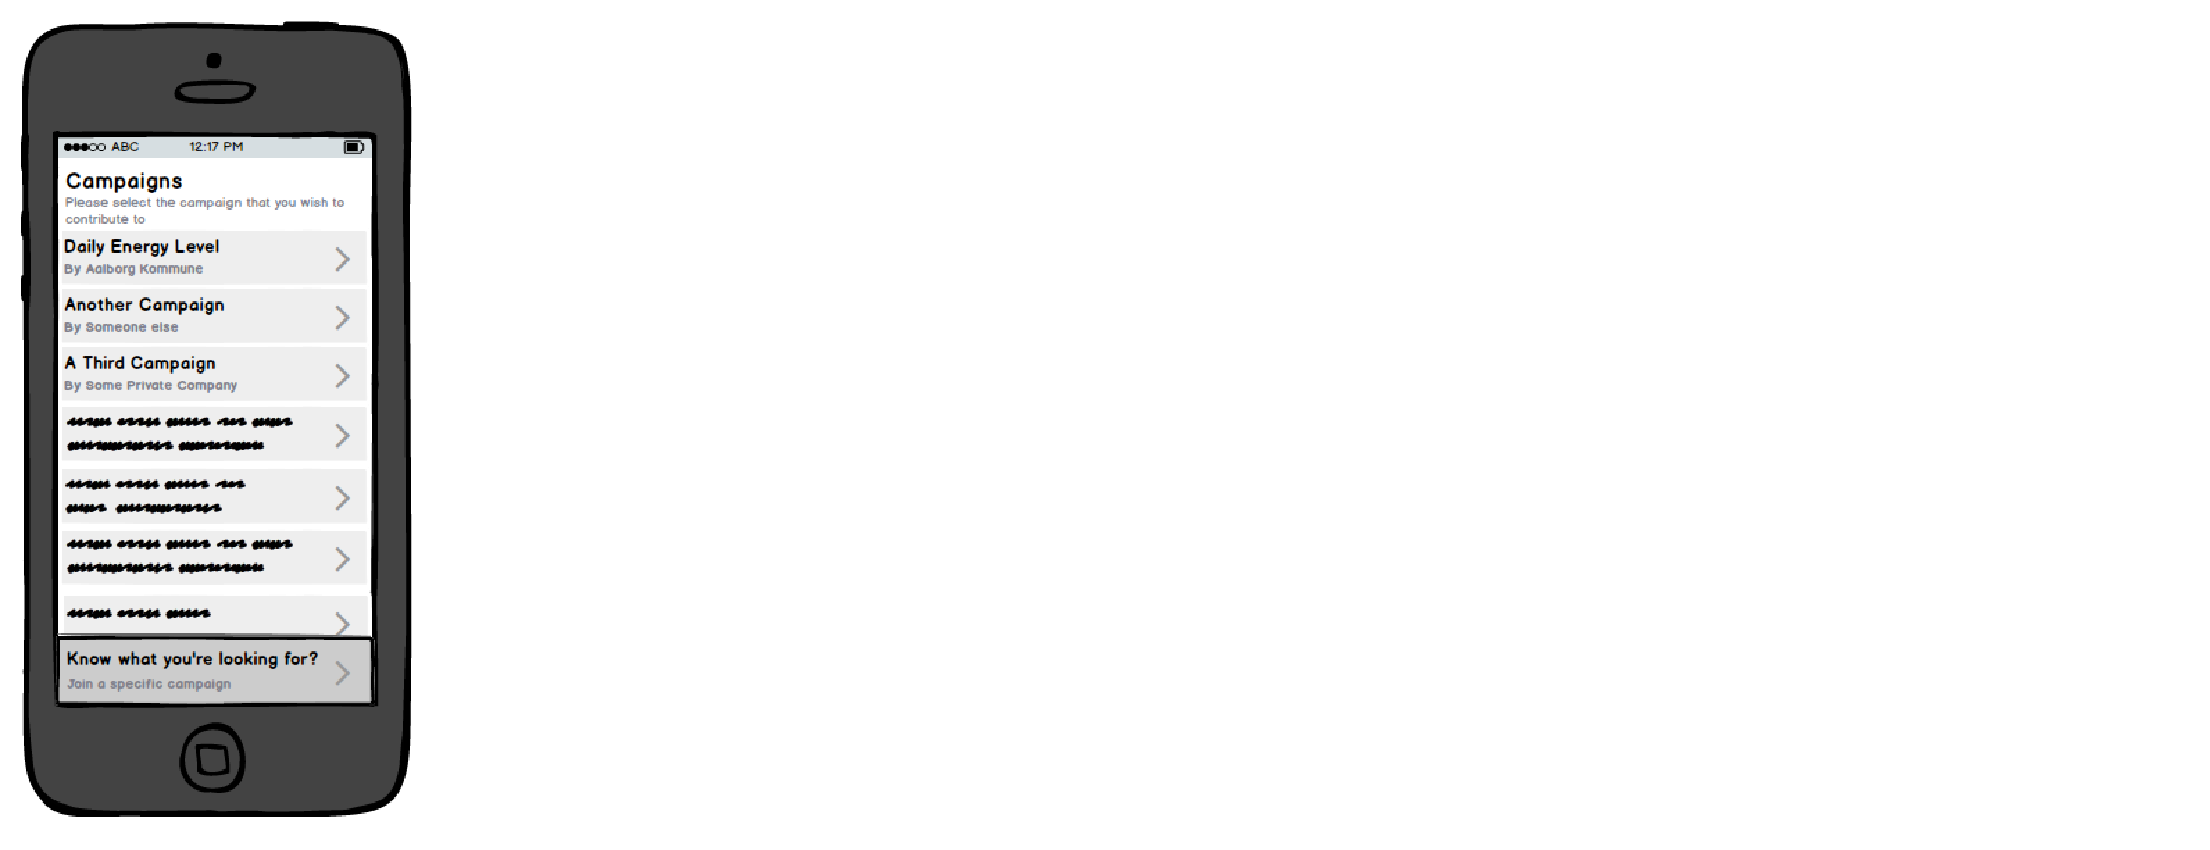
\includegraphics[width=.7\linewidth]{mockups/campaigns_list}
        \caption{Mockup of the browsing view.}
        \label{fig:mockup_public_campaigns}
    \end{subfigure}%
    \begin{subfigure}[!t]{.52\textwidth}
        \centering
        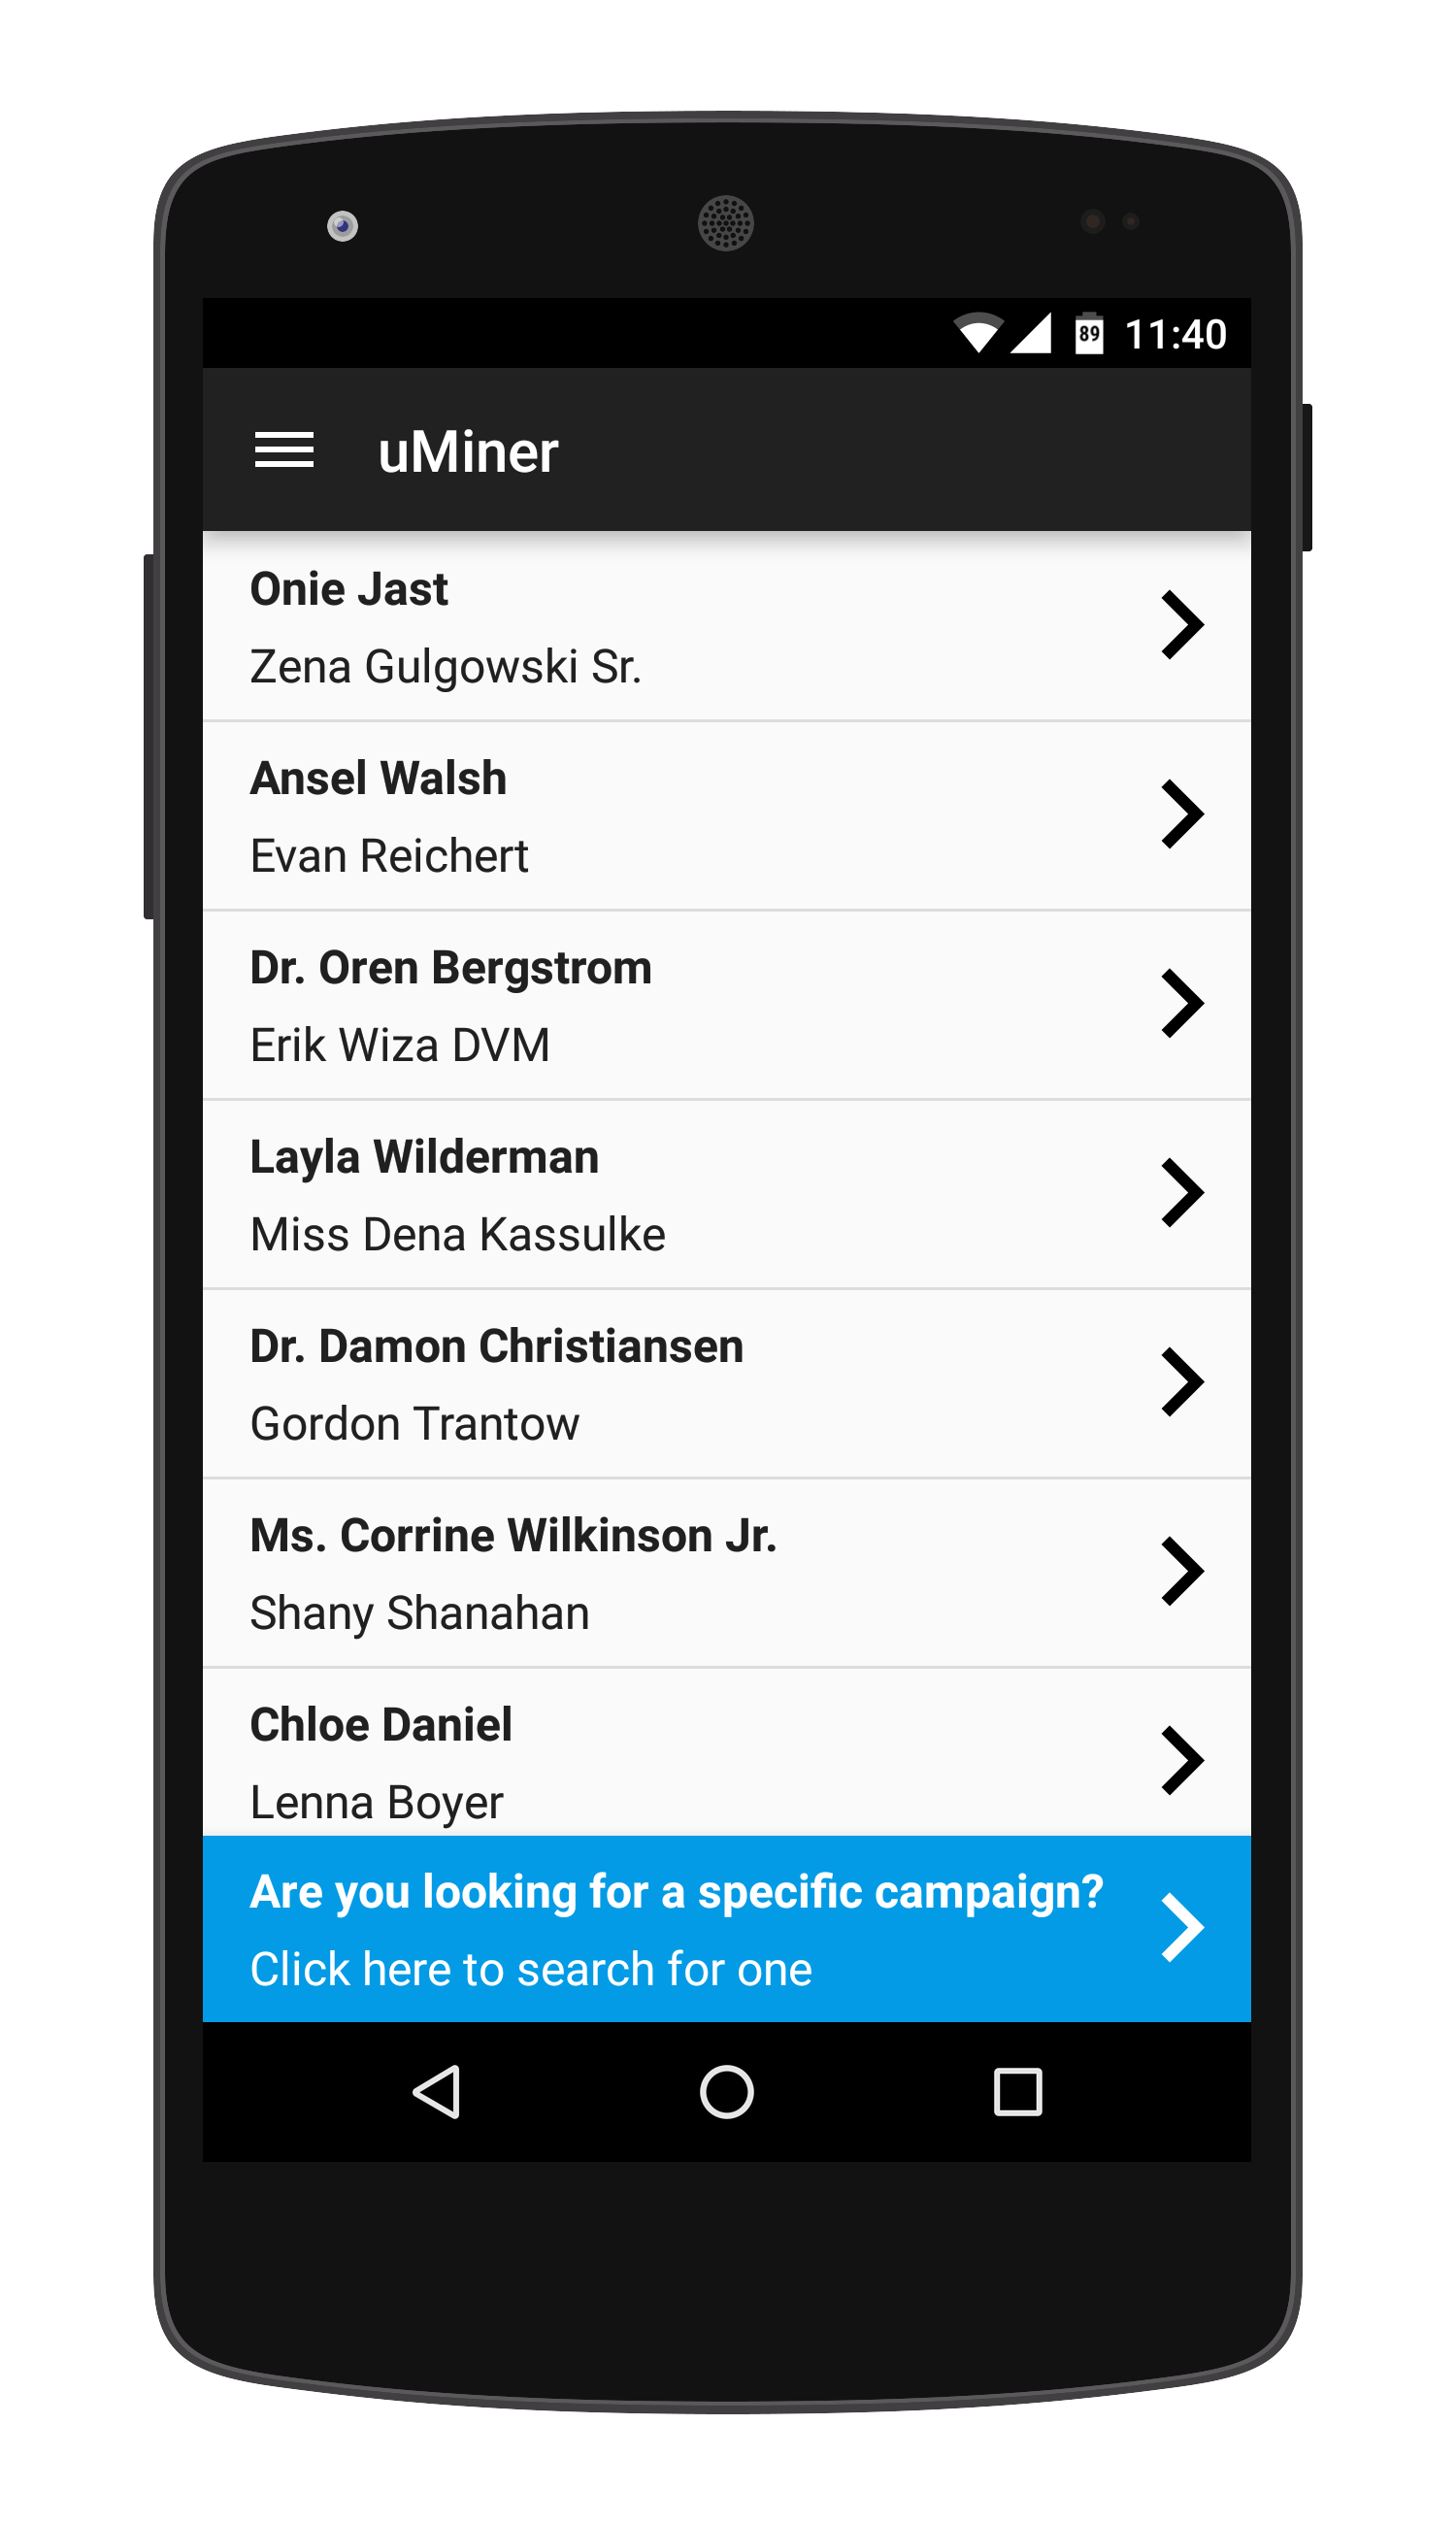
\includegraphics[width=.73\linewidth]{user_interfaces/client/client_public_campaigns_with_phone}
        \caption{Implementation of the browsing view.}
        \label{fig:implementation_public_campaigns}
    \end{subfigure}
    \caption{Mockup and implementation of browsing campaigns.}
    \label{fig:public_campaigns}
\end{figure}
\FloatBarrier

The participant also has the opportunity to join a specific campaign, when browsing the public ones, by pressing the blue area in the bottom, which will always be visible regardless of how far the participant scroll in the list. If the area is pressed, the participant will be redirected to the screen showed in \figref{fig:specific_campaign}. Participants can here enter a unique campaign identifier, if they have been given one by a customer. The participant will, upon entering an identifier, be redirected to a view similar to the one seen in \figref{fig:campaign_specification} if the specified identifier corresponds to a campaign. If not, the participant will be notified that the entered campaign identifier is invalid. 

% Search for a campaign through a campaign identifier
\begin{figure}[!htbp]
    \begin{subfigure}[!t]{.48\textwidth}
        \centering
        
\includegraphics[width=.7\linewidth]{mockups/join_specific_campaign}
        \caption{Mockup for the searching.}
        \label{fig:mockup_specific_campaign}
    \end{subfigure}%
    \begin{subfigure}[!t]{.52\textwidth}
        \centering
        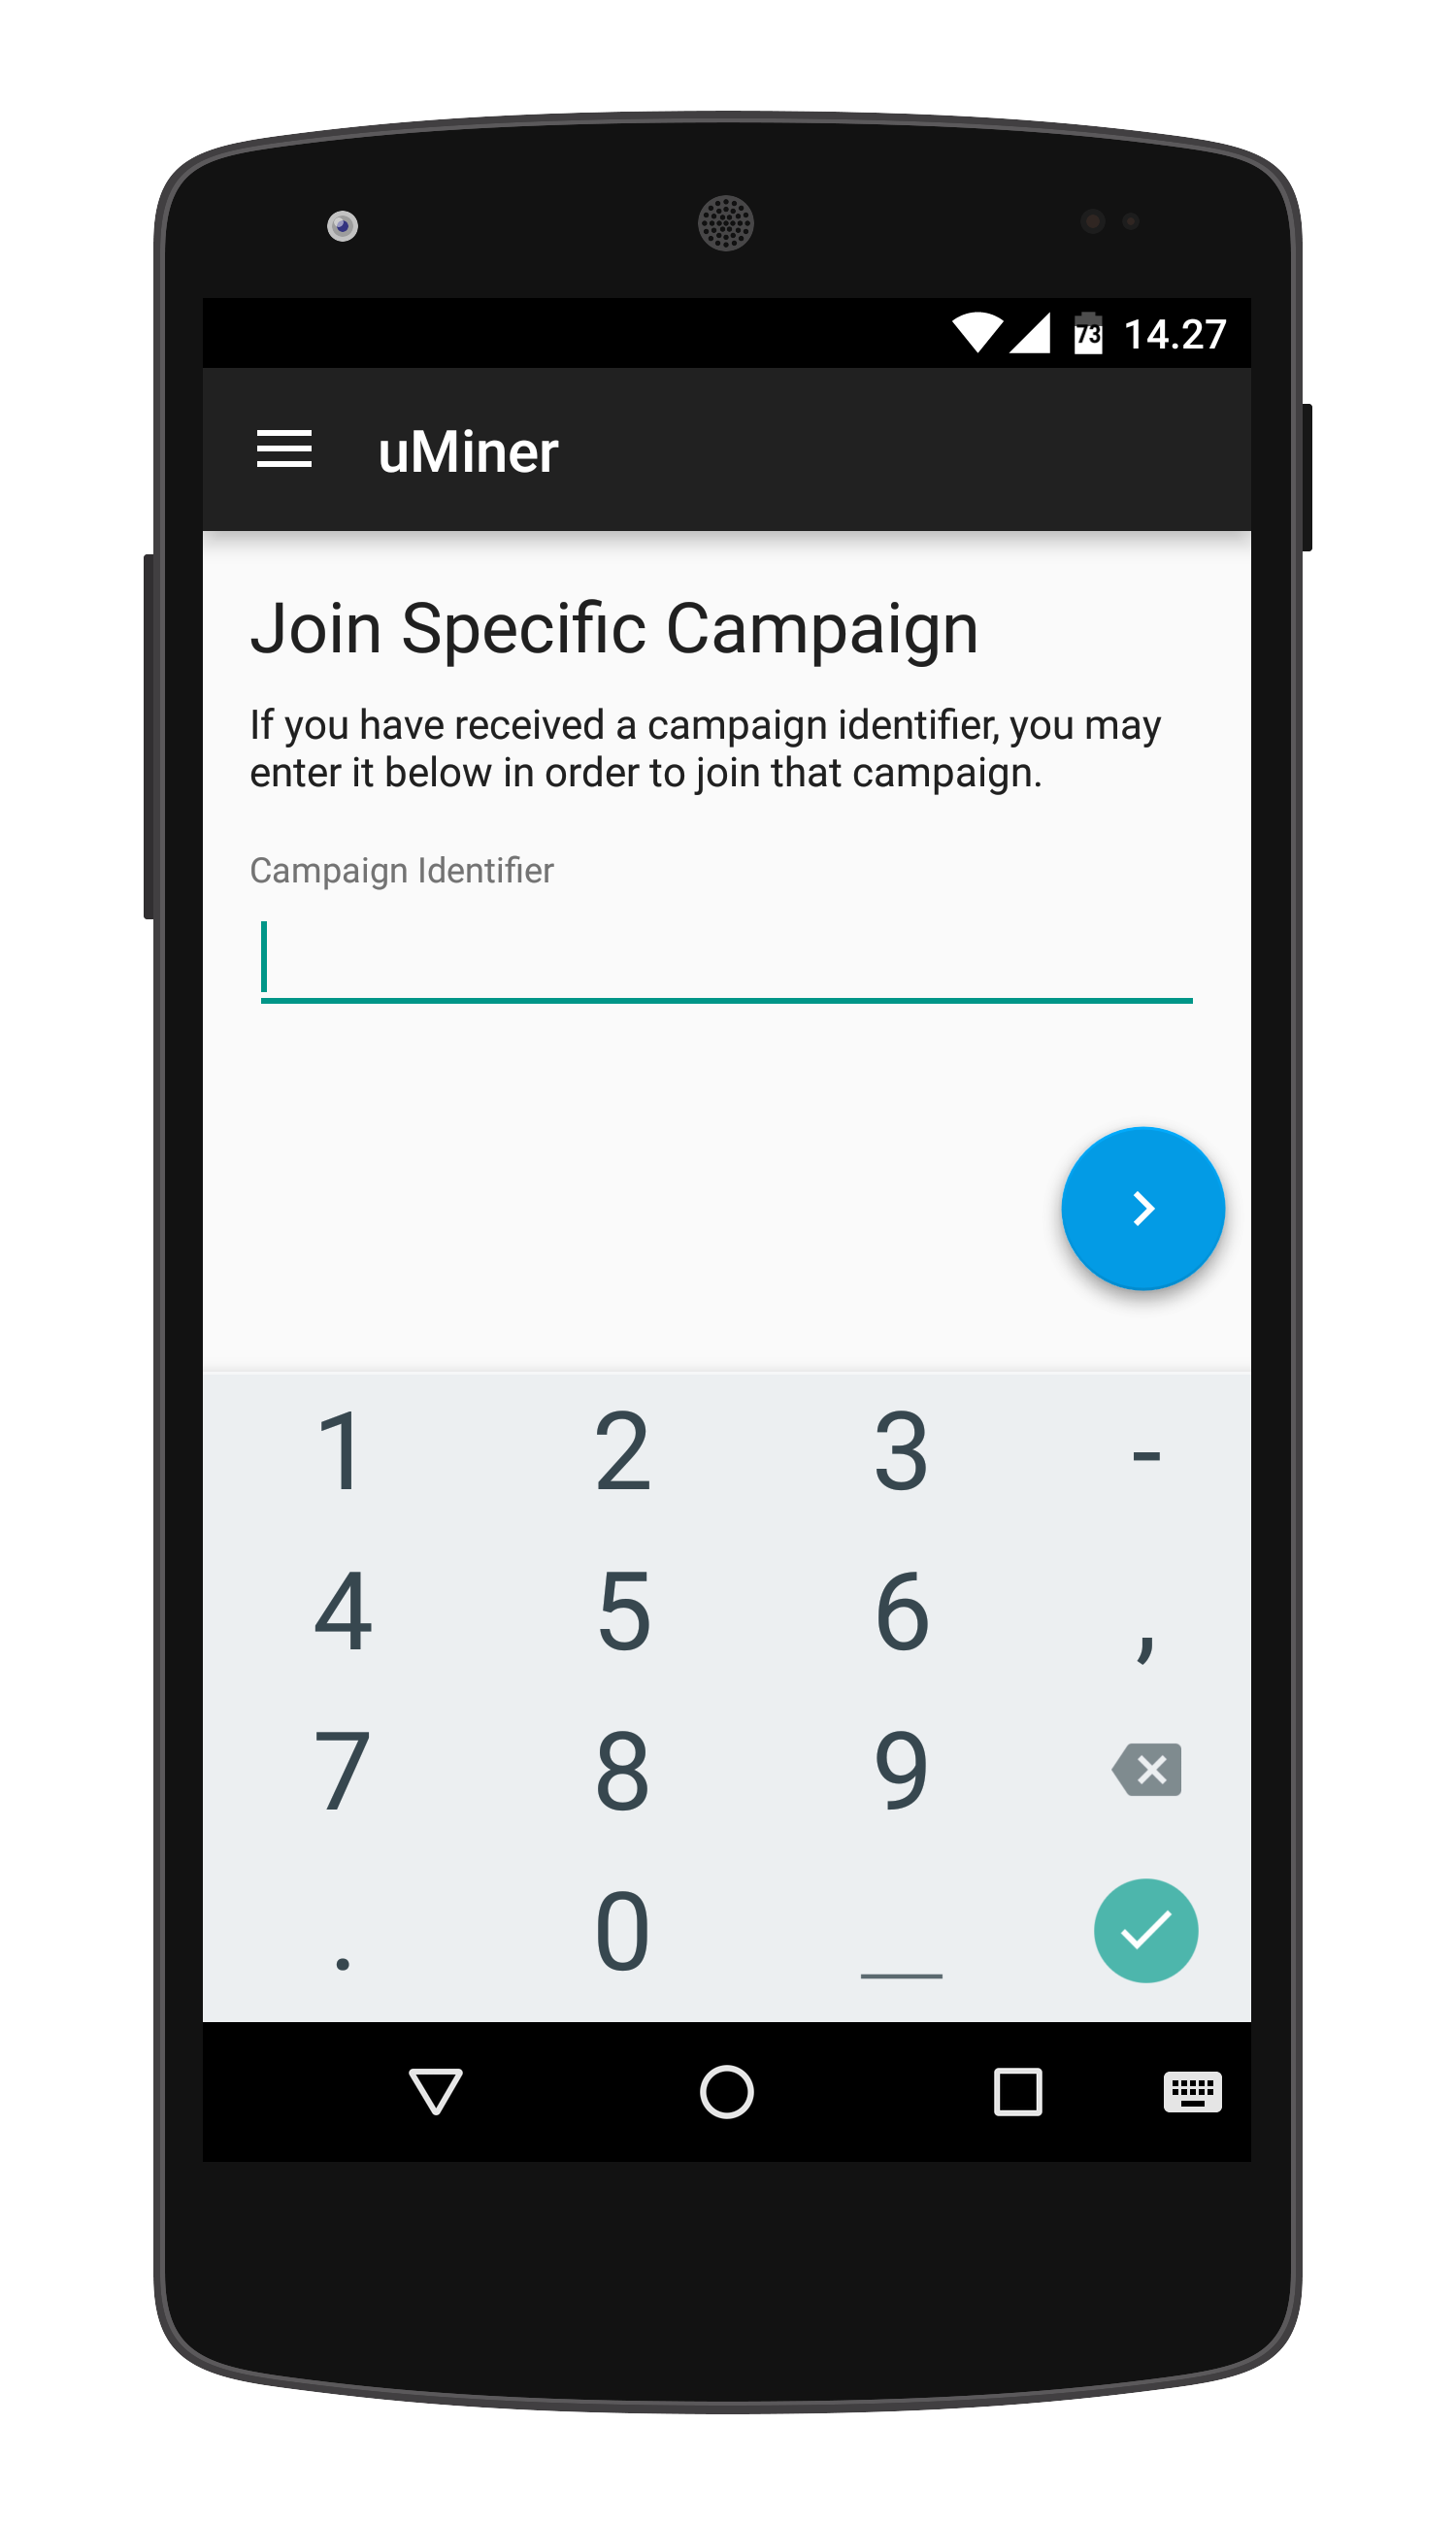
\includegraphics[width=.73\linewidth]{user_interfaces/client/client_join_specific_campaign_with_phone}
        \caption{Implementation for the searching.}
        \label{fig:implementation_specific_campaign}
    \end{subfigure}
    \caption{Mockup and Implementation for searching for a specific campaign using a campaign identifier.}
    \label{fig:specific_campaign}
\end{figure}
\FloatBarrier

The mobile application currently only supports scrolling through the list of public campaigns to find a campaign. One could imagine that at some point in time the amount of campaigns would increase to a number, where it would be infeasible to scroll through. This could be solved by utilizing filtering or querying of campaigns. If this were to be implemented it would be beneficial to do this on the server, such that the device should not download all the information needed to process such queries or filters. Throughout the project period, we have thought of a number of different ways of allowing the participants to find and join campaigns, which could prove to be nice additions to the system, but have not been implemented yet.

\begin{description}
    \item[Quick Response (QR) Codes] could be utilized to give participants an easy way of subscribing to campaigns, by scanning a QR code. Customers would be able to distribute these QR codes through both digital and printed media. Furthermore, QR codes might be more easily relatable for participants, since they might be familiar with the concept from other domains.

    \item[Specific search criteria] might help participants to find exactly what they want to contribute to. Participants might only be willing to contribute to campaigns with a scientific purpose, or campaigns that have next to no impact on battery life. Other criteria might be: limited amount of questions in questionnaires, or none at all. Additionally, some participants might not be willing to contribute to campaigns with specific sensors, e.g. GPS, so the possibility of filtering campaigns by different sensors might also be desirable.

    \item[Prizes and other motivational factors] are not present in the current state of the system. However, if they were to be introduced, they would potentially have a big impact on which campaigns gets contributed to. This means that the application could assist customers in getting more participants for their campaigns by displaying information regarding the prizes that customers provide to contributing participants. One could also imagine that participants could filter campaigns depending on whether they provide a reward or not.
\end{description} 

\subsection{Contributing to Campaigns}
\label{sub:contributing_to_campaigns}

To contribute to a specific campaign, participants must firstly find a campaign that they want to contribute to. This can be done through the campaign browser, previously shown in \figref{fig:public_campaigns}, or entering a unique identifier in the join specific campaign screen, previously shown in \figref{fig:specific_campaign}. The participants must then navigate to a campaign specification screen, similar to the one seen in \figref{fig:campaign_specification}. 
\\\\
After a participant has found a campaign that he is willing to contribute to, he will find himself/herself on an overview of the information related to the campaign in a view similar to the one seen in \figref{fig:campaign_specification}. After reviewing this information, the participant can decide if he wants to contribute by subscribing to the campaign, which will be done by pressing the green subscribe button. This will signal the background service to start the collection of snapshots as described in \secref{sub:background_sensor_service_snapshot_generation_and_synchronization}.

% Campaign specification
\begin{figure}[!htbp]
    \begin{subfigure}[!t]{.48\textwidth}
        \centering
        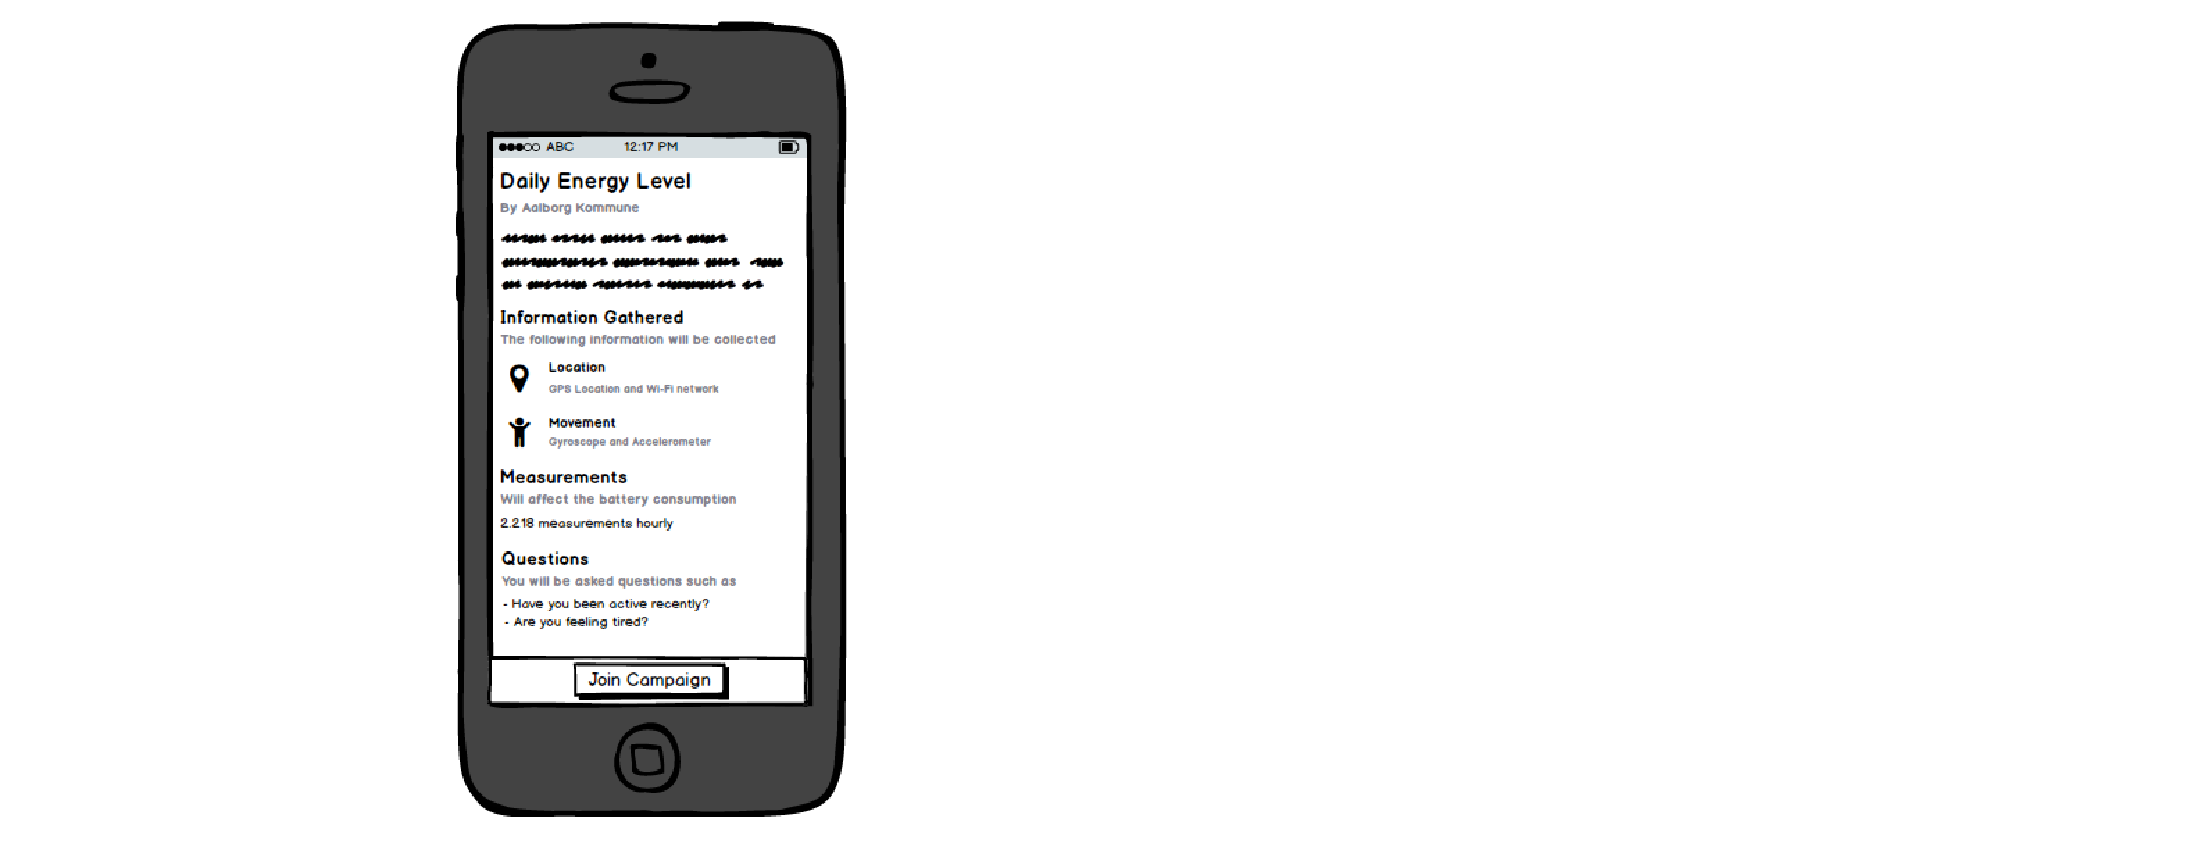
\includegraphics[width=.7\linewidth]{mockups/campaign_specification}
        \caption{Mockup of the specification screen.}
        \label{fig:mockup_campaign_specification}
    \end{subfigure}%
    \begin{subfigure}[!t]{.52\textwidth}
        \centering
        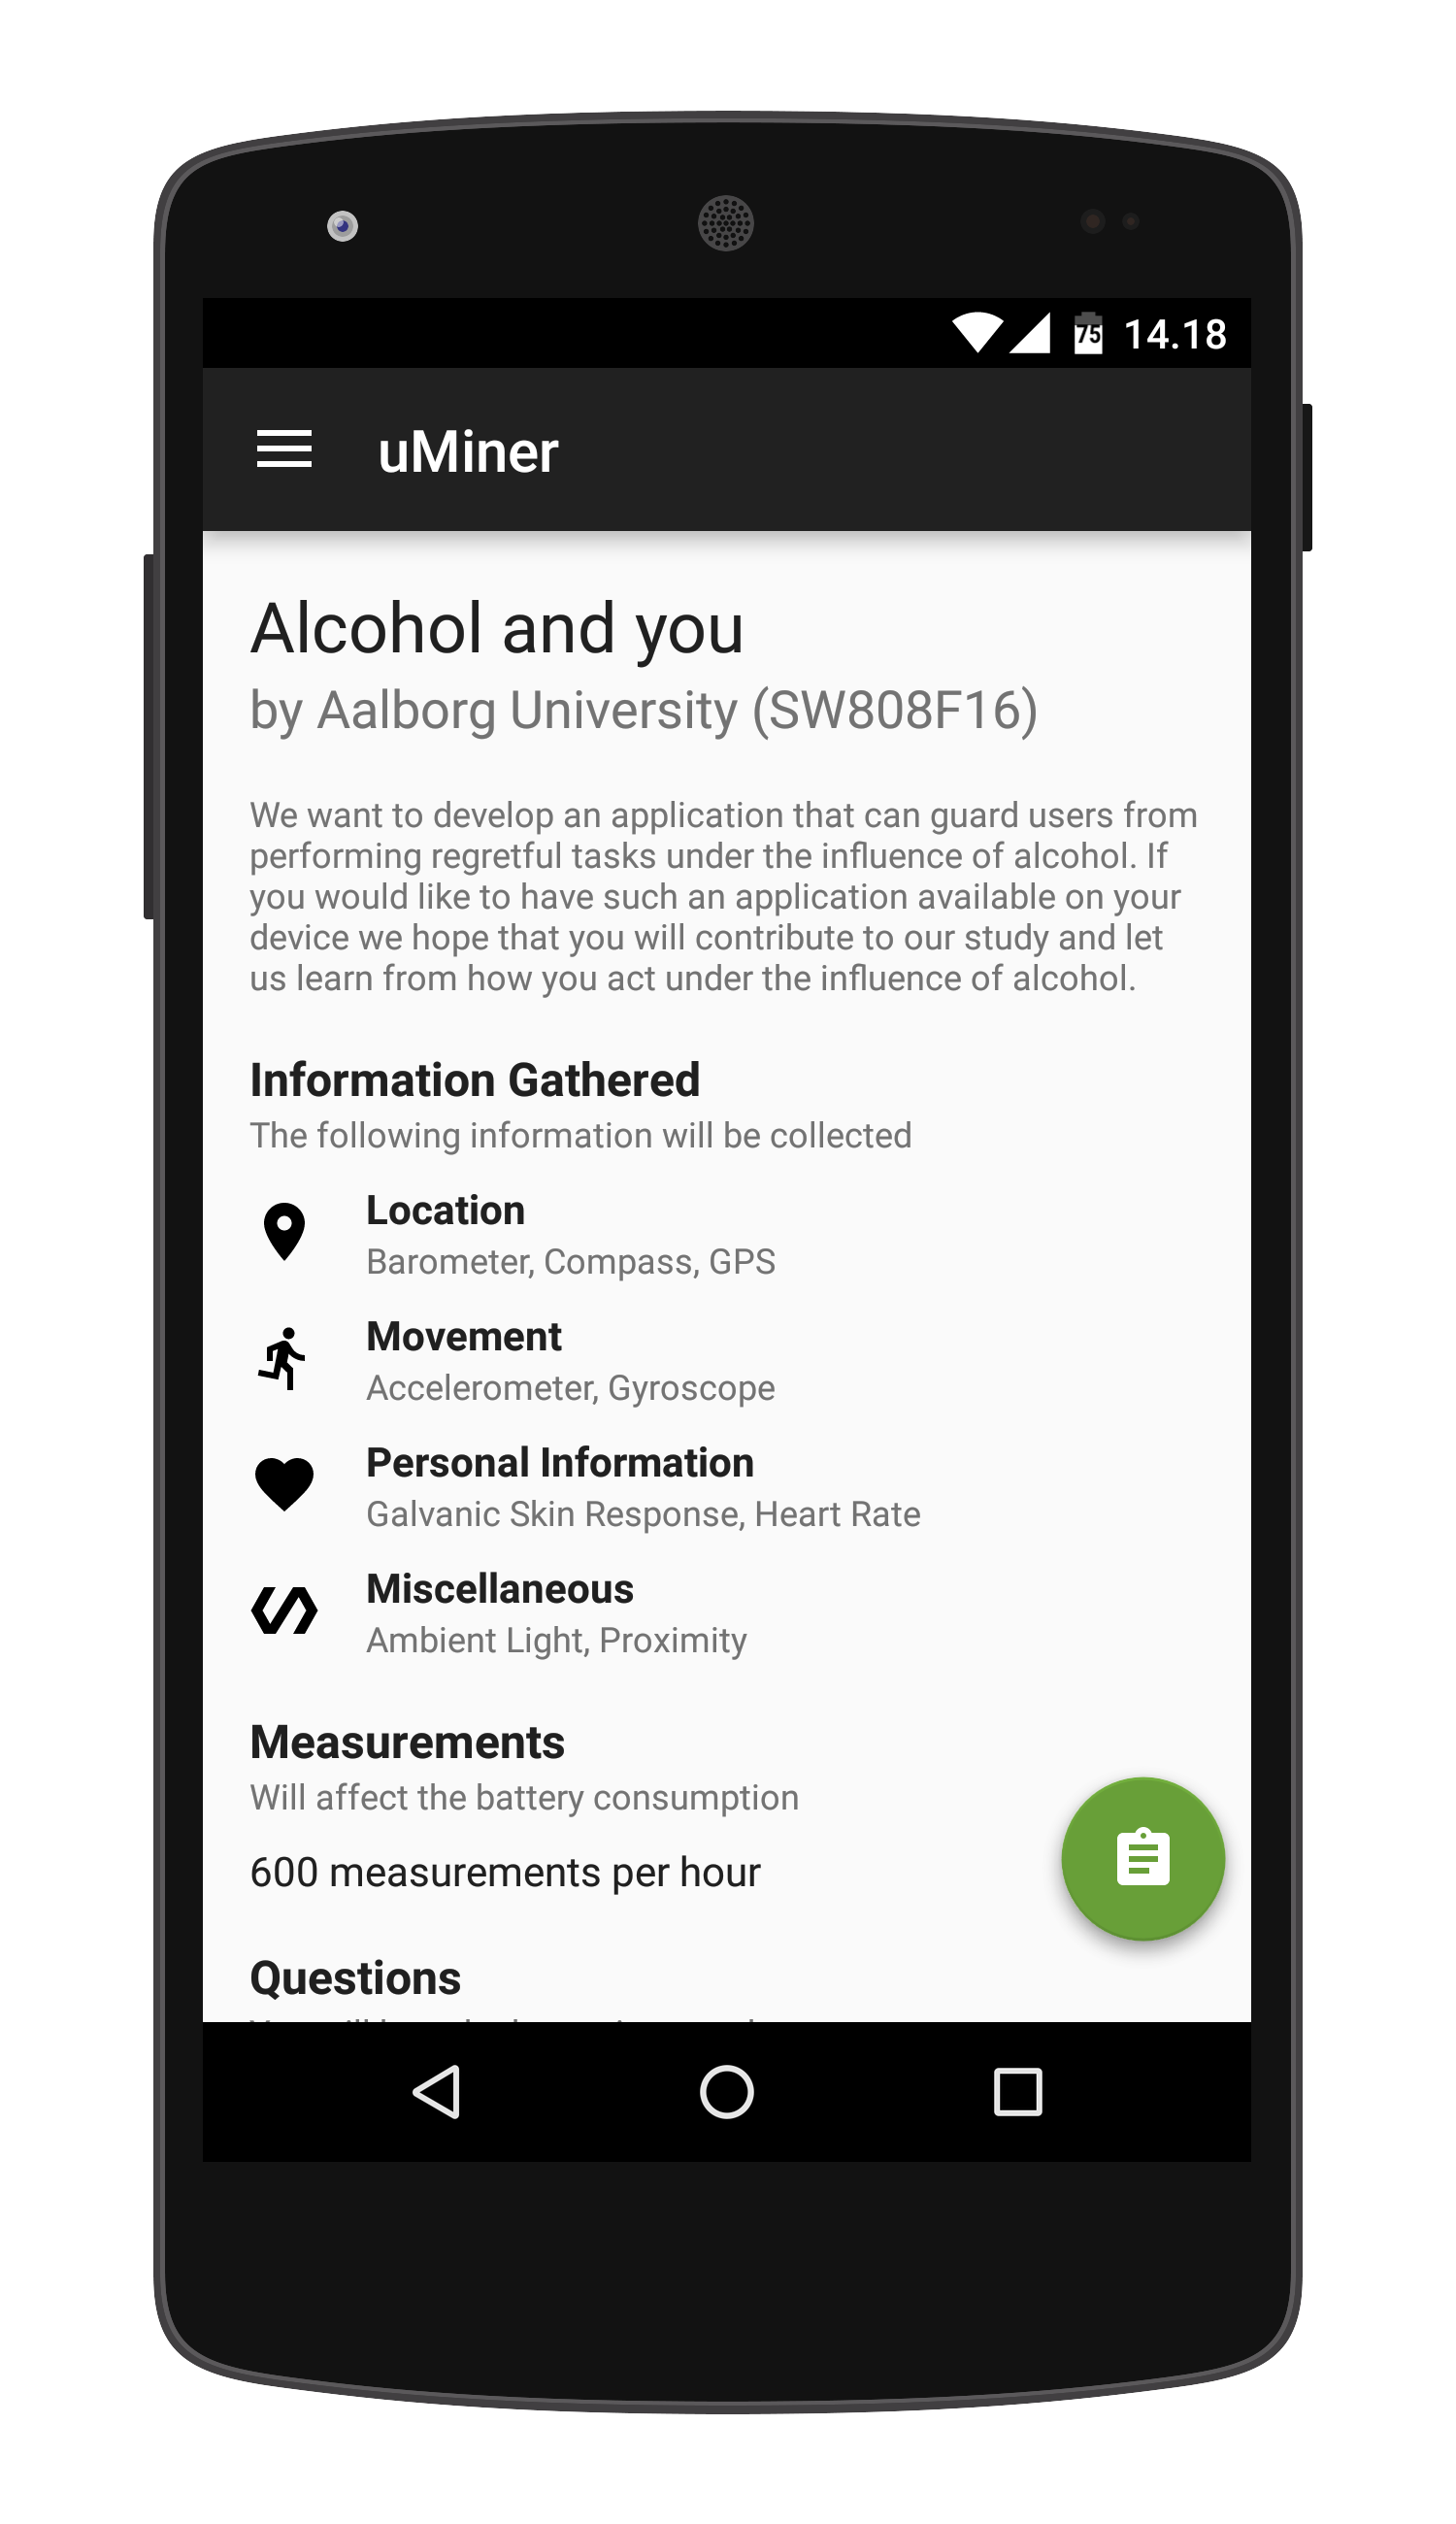
\includegraphics[width=.73\linewidth]{user_interfaces/client/client_campaign_specification2_with_phone}
        \caption{Implementation of the specification screen.}
        \label{fig:implementation_campaign_specification}
    \end{subfigure}
    \caption{Mockup and implementation of the specification screen for a campaign.}
    \label{fig:campaign_specification}
\end{figure}
\FloatBarrier

If for any reason, a participant no longer wishes to contribute to a campaign, he can navigate to the specification for the given campaign. This time, the otherwise green subscribe button will instead be a red unsubscribe button, as seen in \figref{fig:leave_campaign_no_dialog}. Pressing this button, will prompt the participant with a confirmation dialog, as seen in \figref{fig:leave_campaign_dialog}. If the participant confirms the action, by pressing yes, the background sensor service is signaled to stop generating snapshots. However, the snapshot currently being generated will complete and be uploaded to the server. This happens because the service (described in \secref{sec:background_sensor_service}) that starts the sensor gathering does not have a hook on the threads that produces output from sensors, and for that reason it is, in the current state of uMiner, not possible to stop the gathering immediately.

% Leave campaign and dialog
\begin{figure}[!htbp]
    \begin{subfigure}[!t]{.50\textwidth}
        \centering
        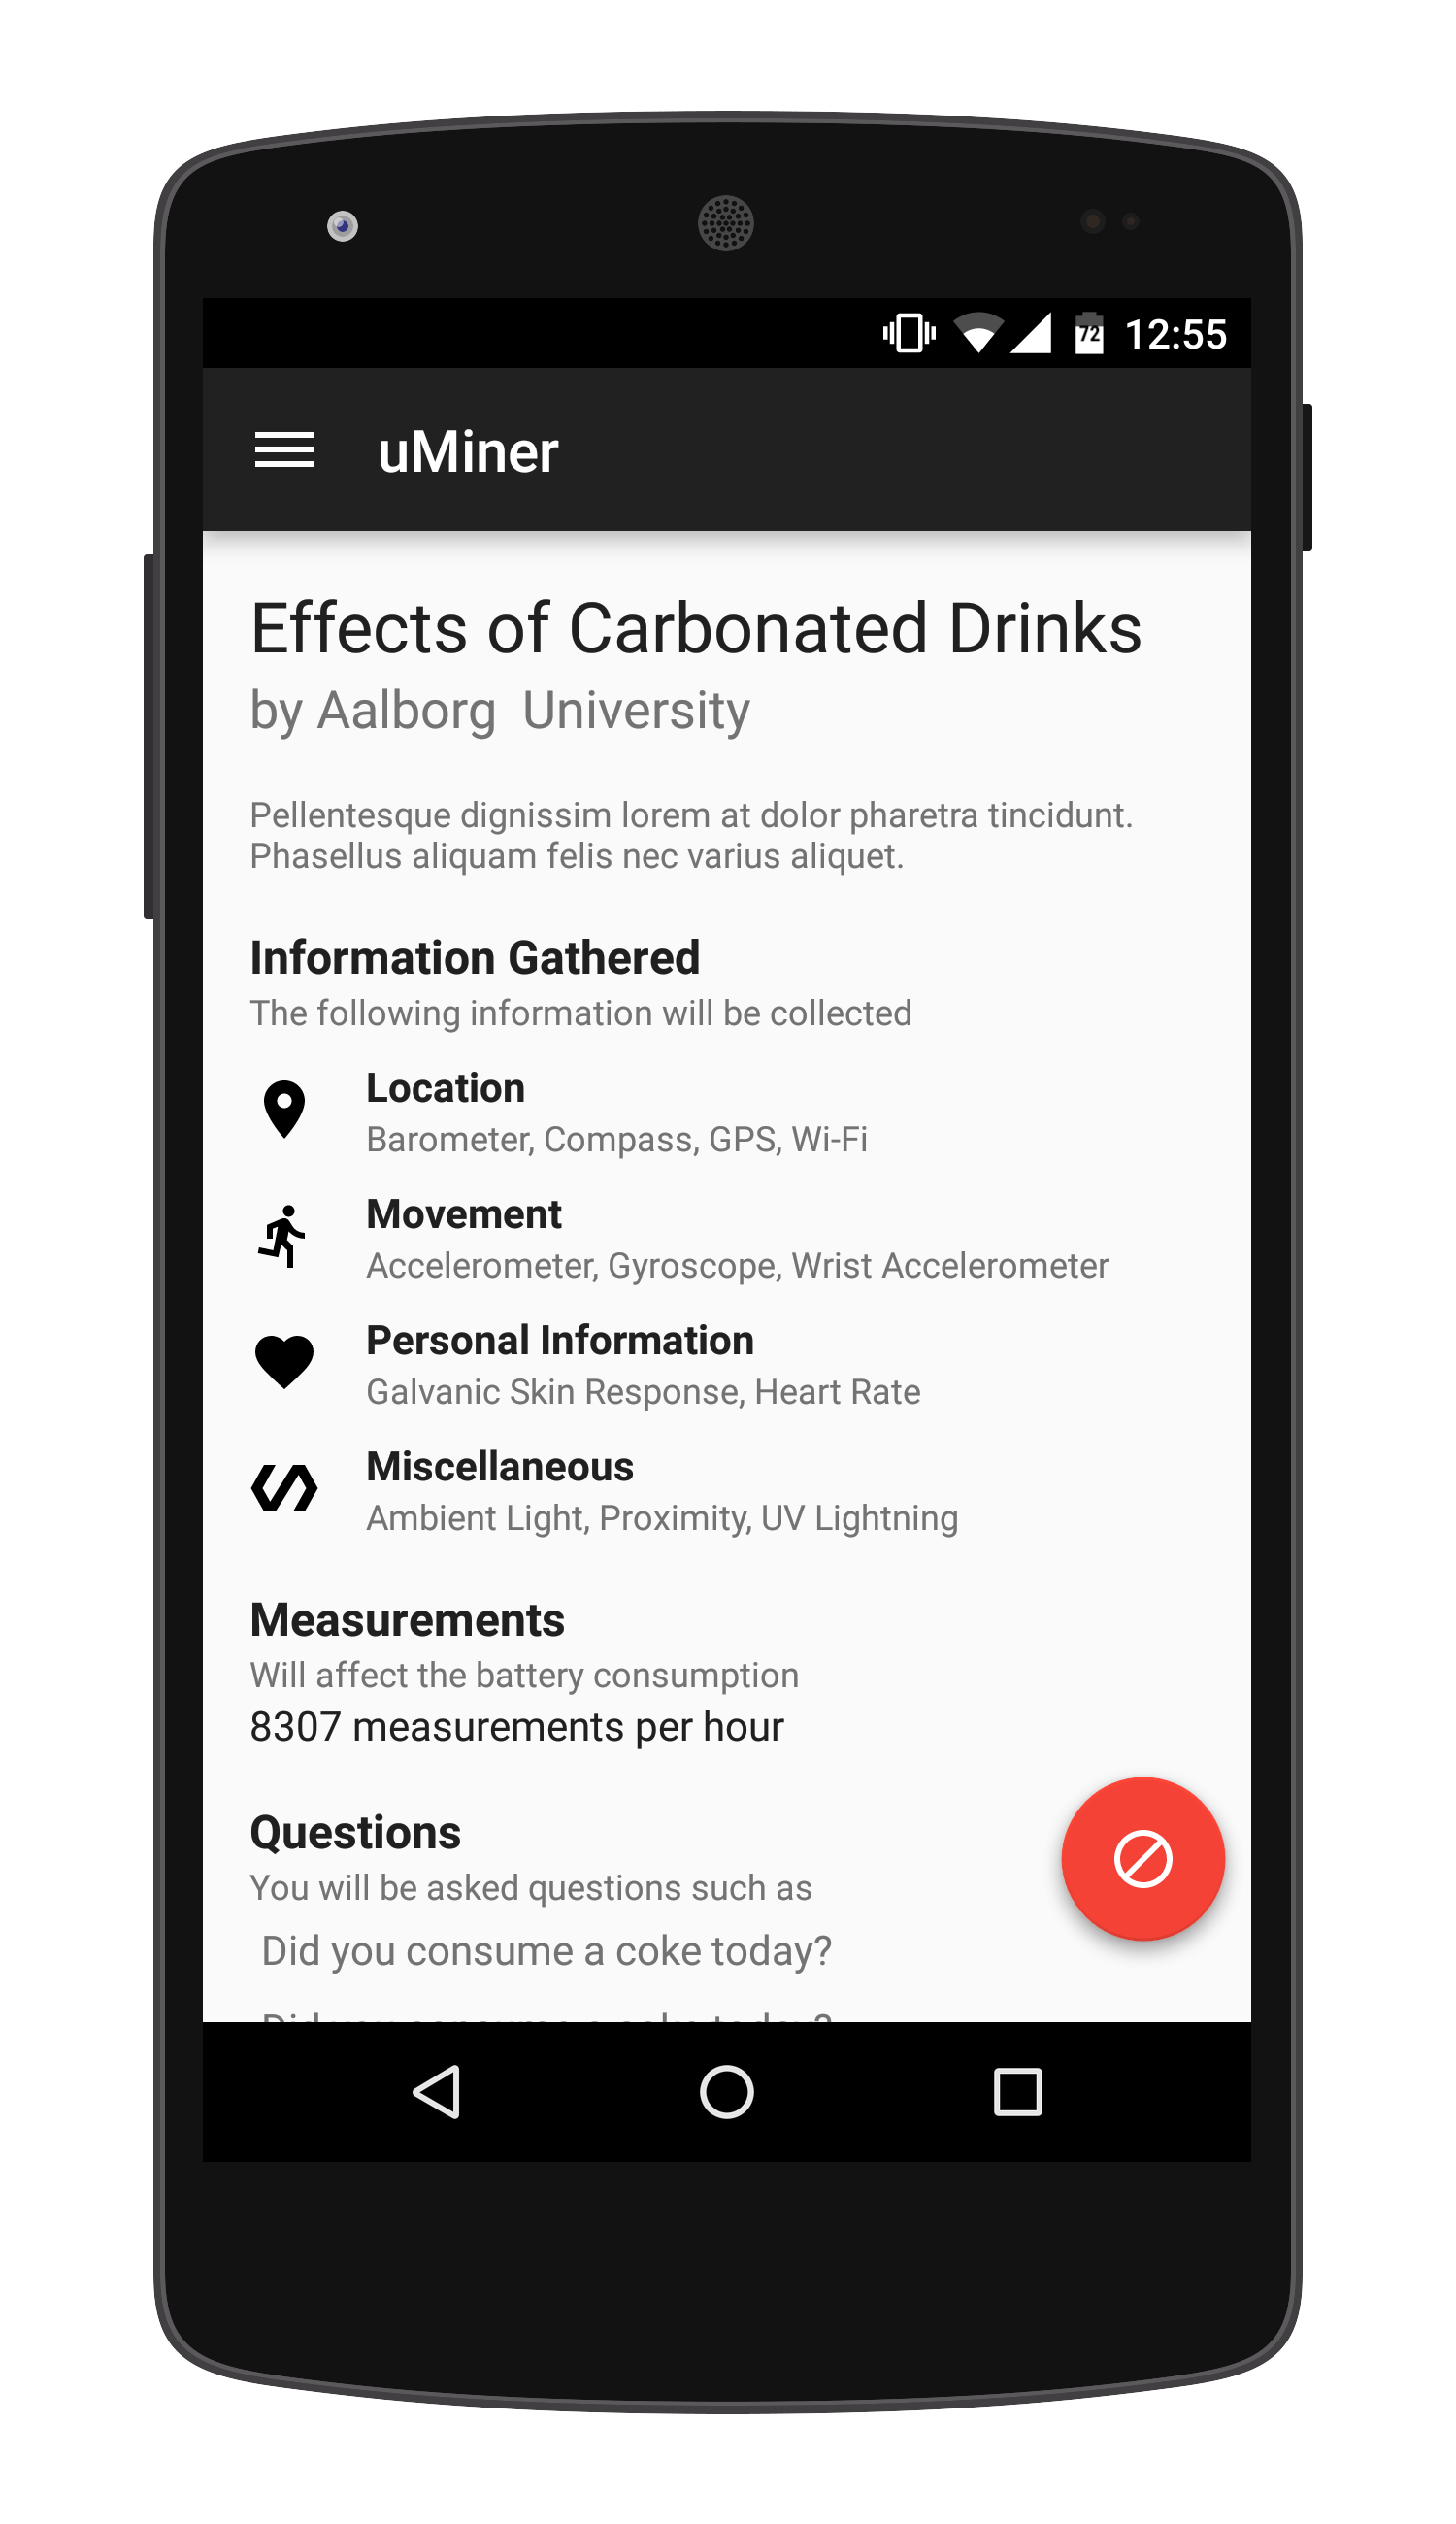
\includegraphics[width=.73\linewidth]{user_interfaces/client/client_leave_campaign_no_dialog_with_phone}
        \caption{Specification screen with an unsubscribe \\\hspace{\textwidth}button.}
        \label{fig:leave_campaign_no_dialog}
    \end{subfigure}%
    \begin{subfigure}[!t]{.50\textwidth}
        \centering
        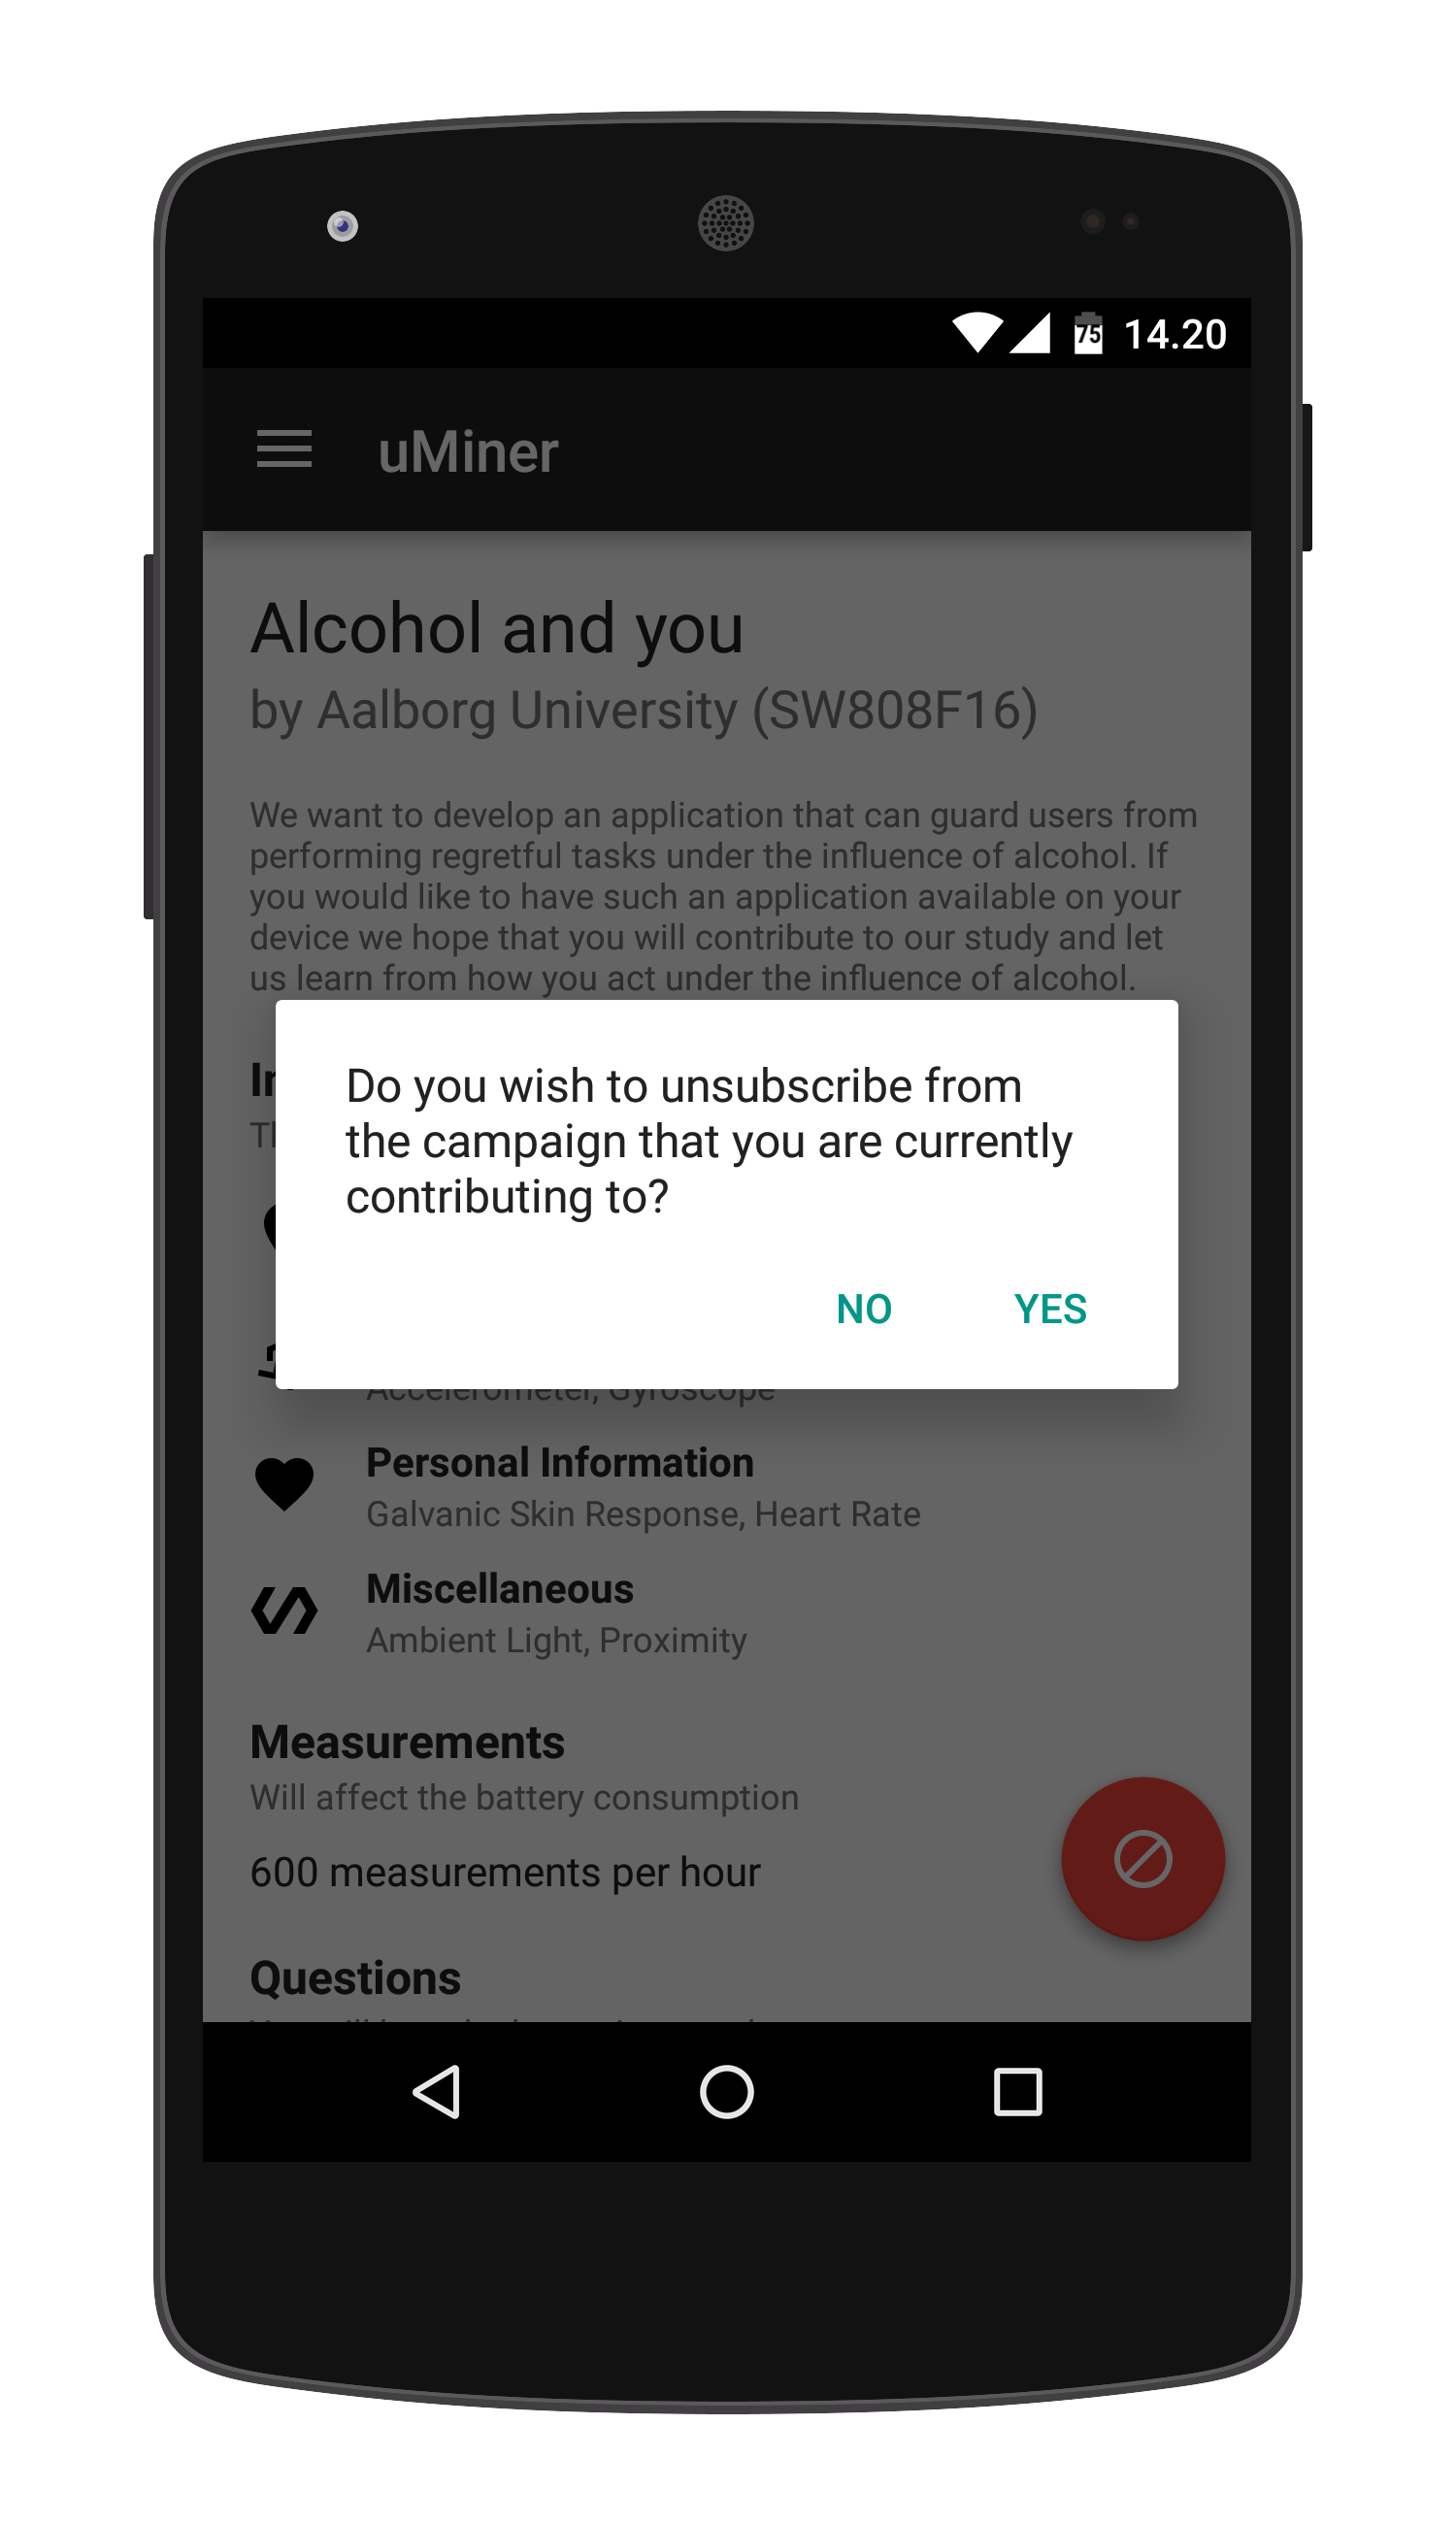
\includegraphics[width=.73\linewidth]{user_interfaces/client/client_leave_campaign_with_phone}
        \caption{Confirmation dialog triggered by pressing the unsubscribe button.}
        \label{fig:leave_campaign_dialog}
    \end{subfigure}
    \caption{Specification screen of a campaign when a participant has joined it.}
    \label{fig:leave_campaign}
\end{figure}
\FloatBarrier

\subsection{Answering Questionnaires}
\label{sub:answering_questionnaired}
% This complies with the way we intended the system to work regarding the participatory sensing as described in \secref{sec:human_activity_recognition}\todo{er det her godt nok?}.
A participant will be requested to answer questionnaires. These request can occur at any time, even at times where the participant is not actively using uMiner. We have chosen to use Android notifications \parencite{android_notifications} to facilitate these request to participants. A notification will then pop-up when a participant should answer questionnaires, as can be seen in \figref{fig:answering_questionnaire_notification}. One benefit of using Android notifications is, that it allows participants some degree of configuration of how and to which degree they want to be disturbed. Android includes global settings which affects how notifications are delivered to its users. The participants can in this way configure a downtime where they do not wish to be disturbed, for instance when they are at work. Notifications in Android also allows users to configure different sound levels or activate silent mode to minimize disturbances for a period. Our application thus synergizes well with a general usage pattern in Android.     
\\\\
When a notification is pressed, the application opens the questionnaire screen as seen in \figref{fig:answering_questionnaire_answering}. We have tried to keep this view simple to allow the participants to quickly answer the questionnaire without any distraction. When the questionnaire is completed the participants will be redirected back to what they were doing before to make the experience of answering questionnaires seamless. 
% Answering questionnaires
\begin{figure}[!htbp]
    \begin{subfigure}[!t]{.50\textwidth}
        \centering
        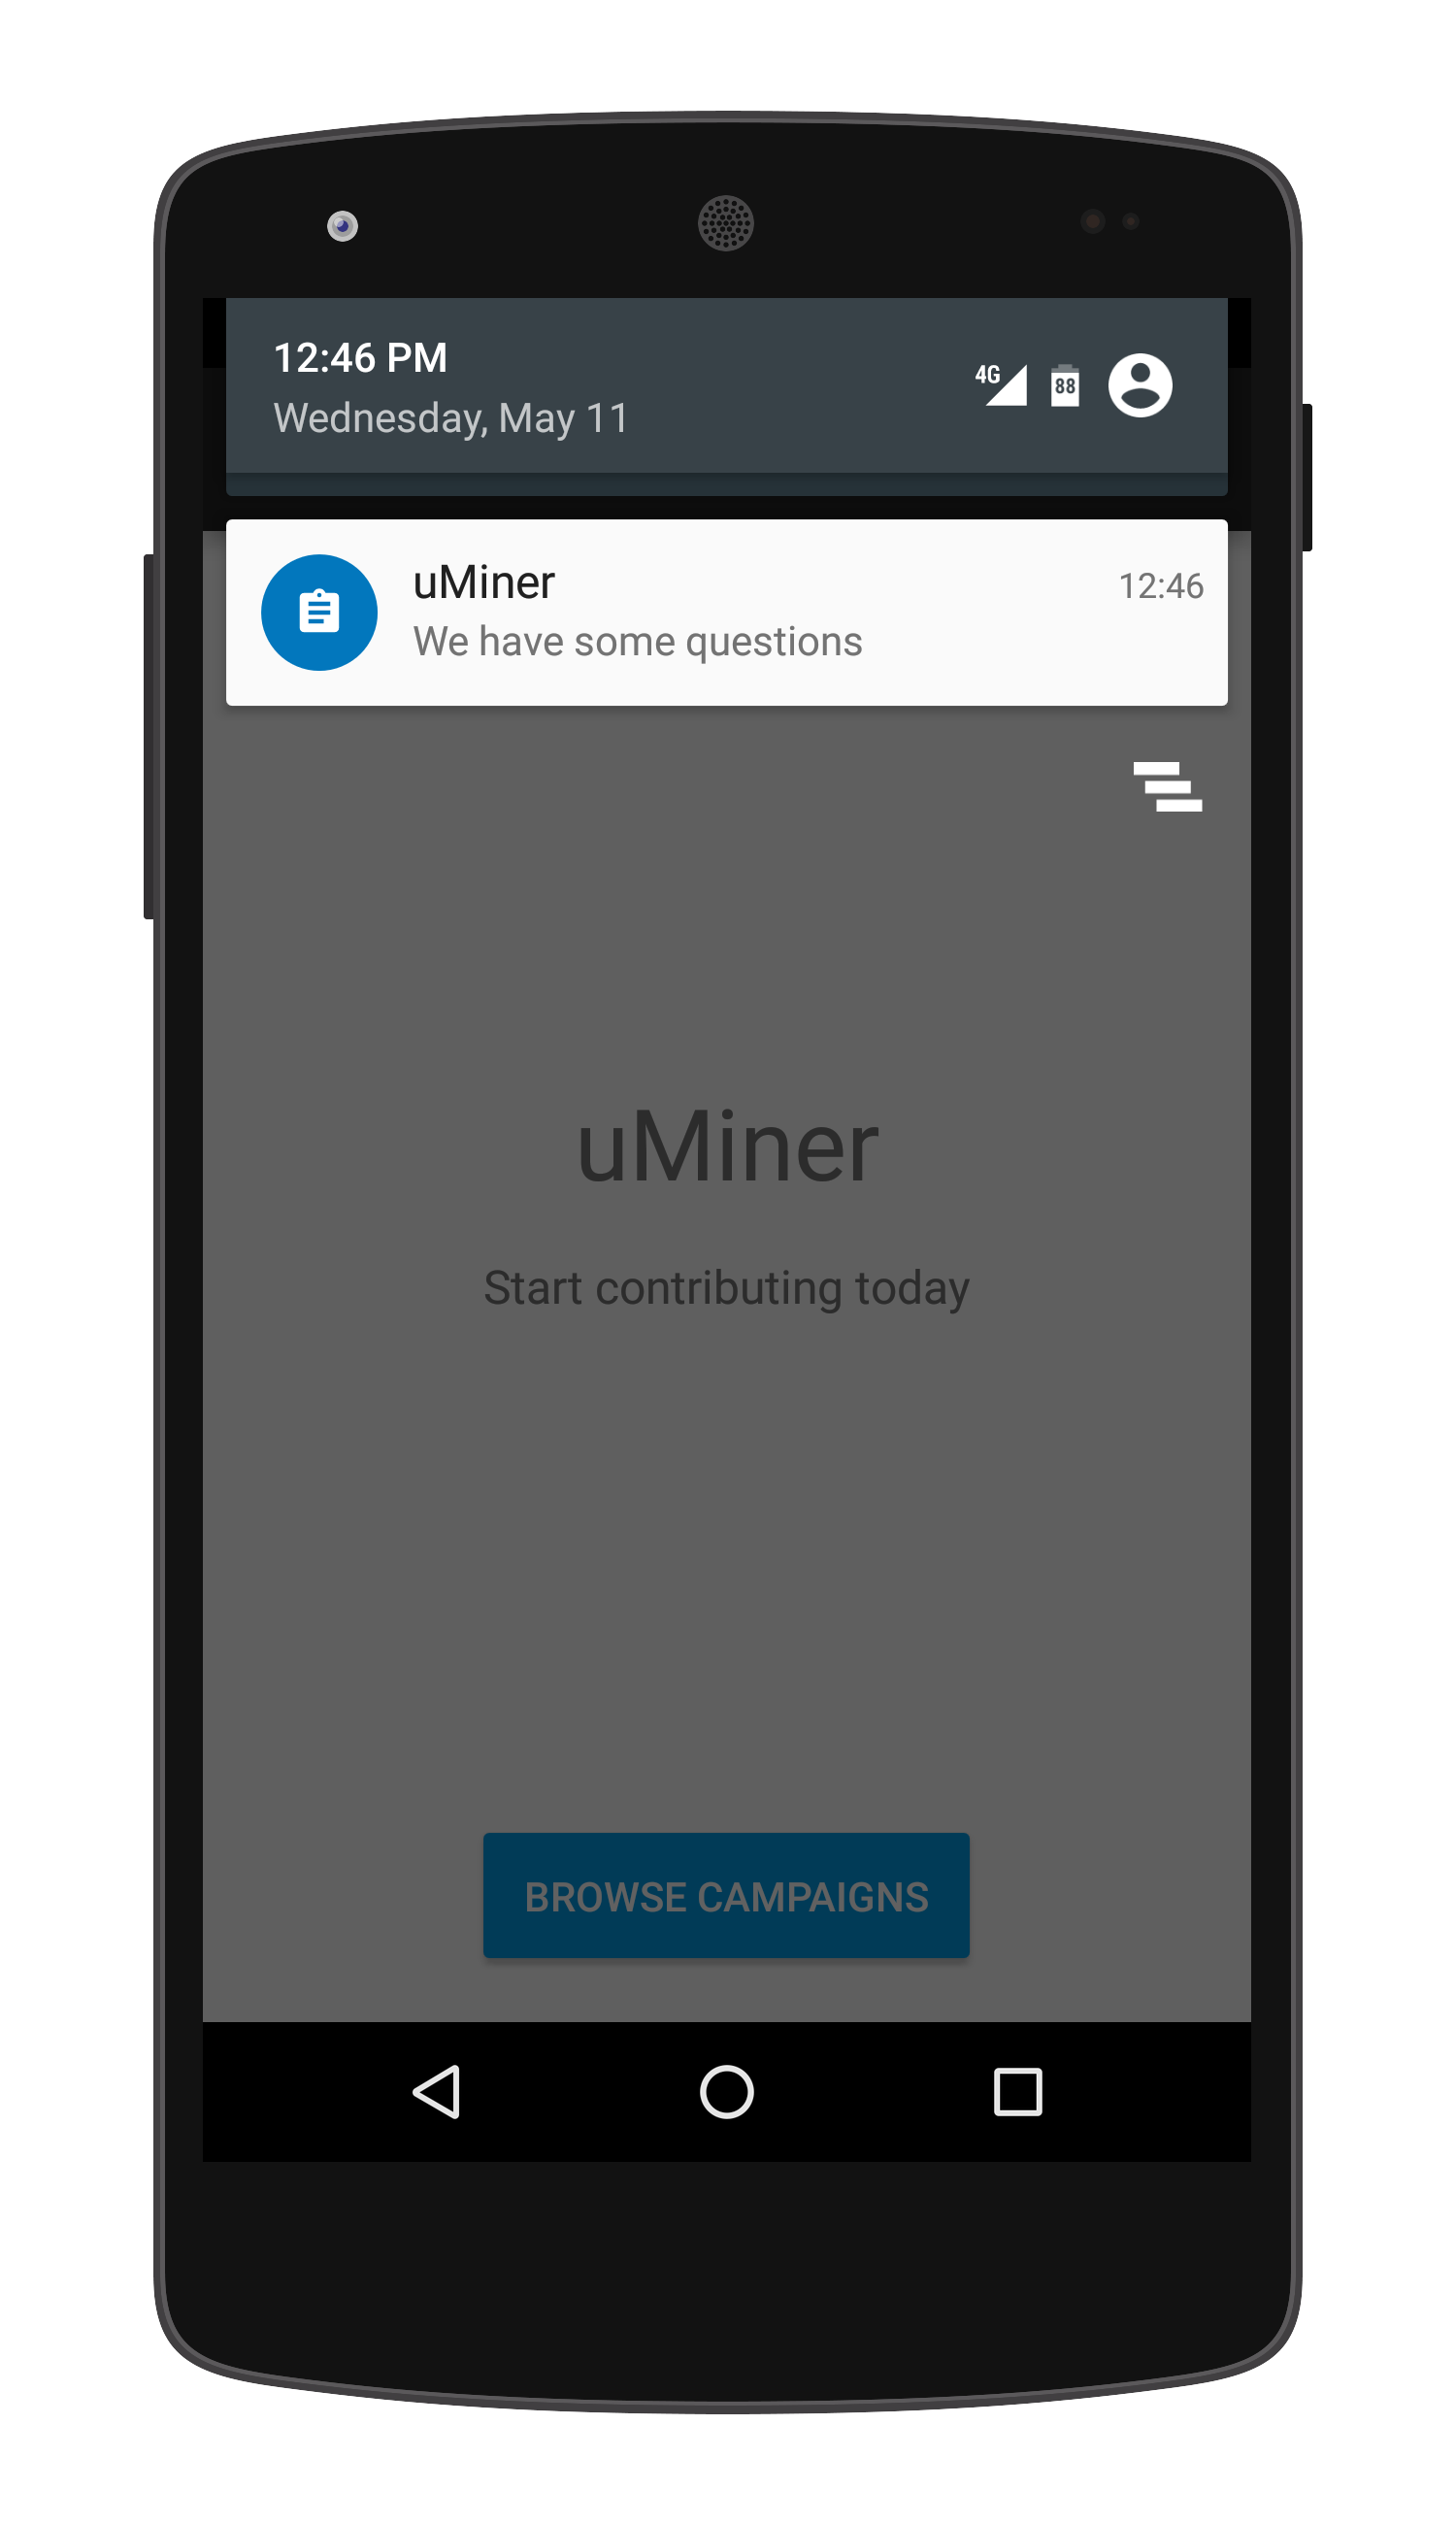
\includegraphics[width=.73\linewidth]{user_interfaces/client/client_notification_with_phone}
        \caption{Notification to answer questions.}
        \label{fig:answering_questionnaire_notification}
    \end{subfigure}%
    \begin{subfigure}[!t]{.50\textwidth}
        \centering
        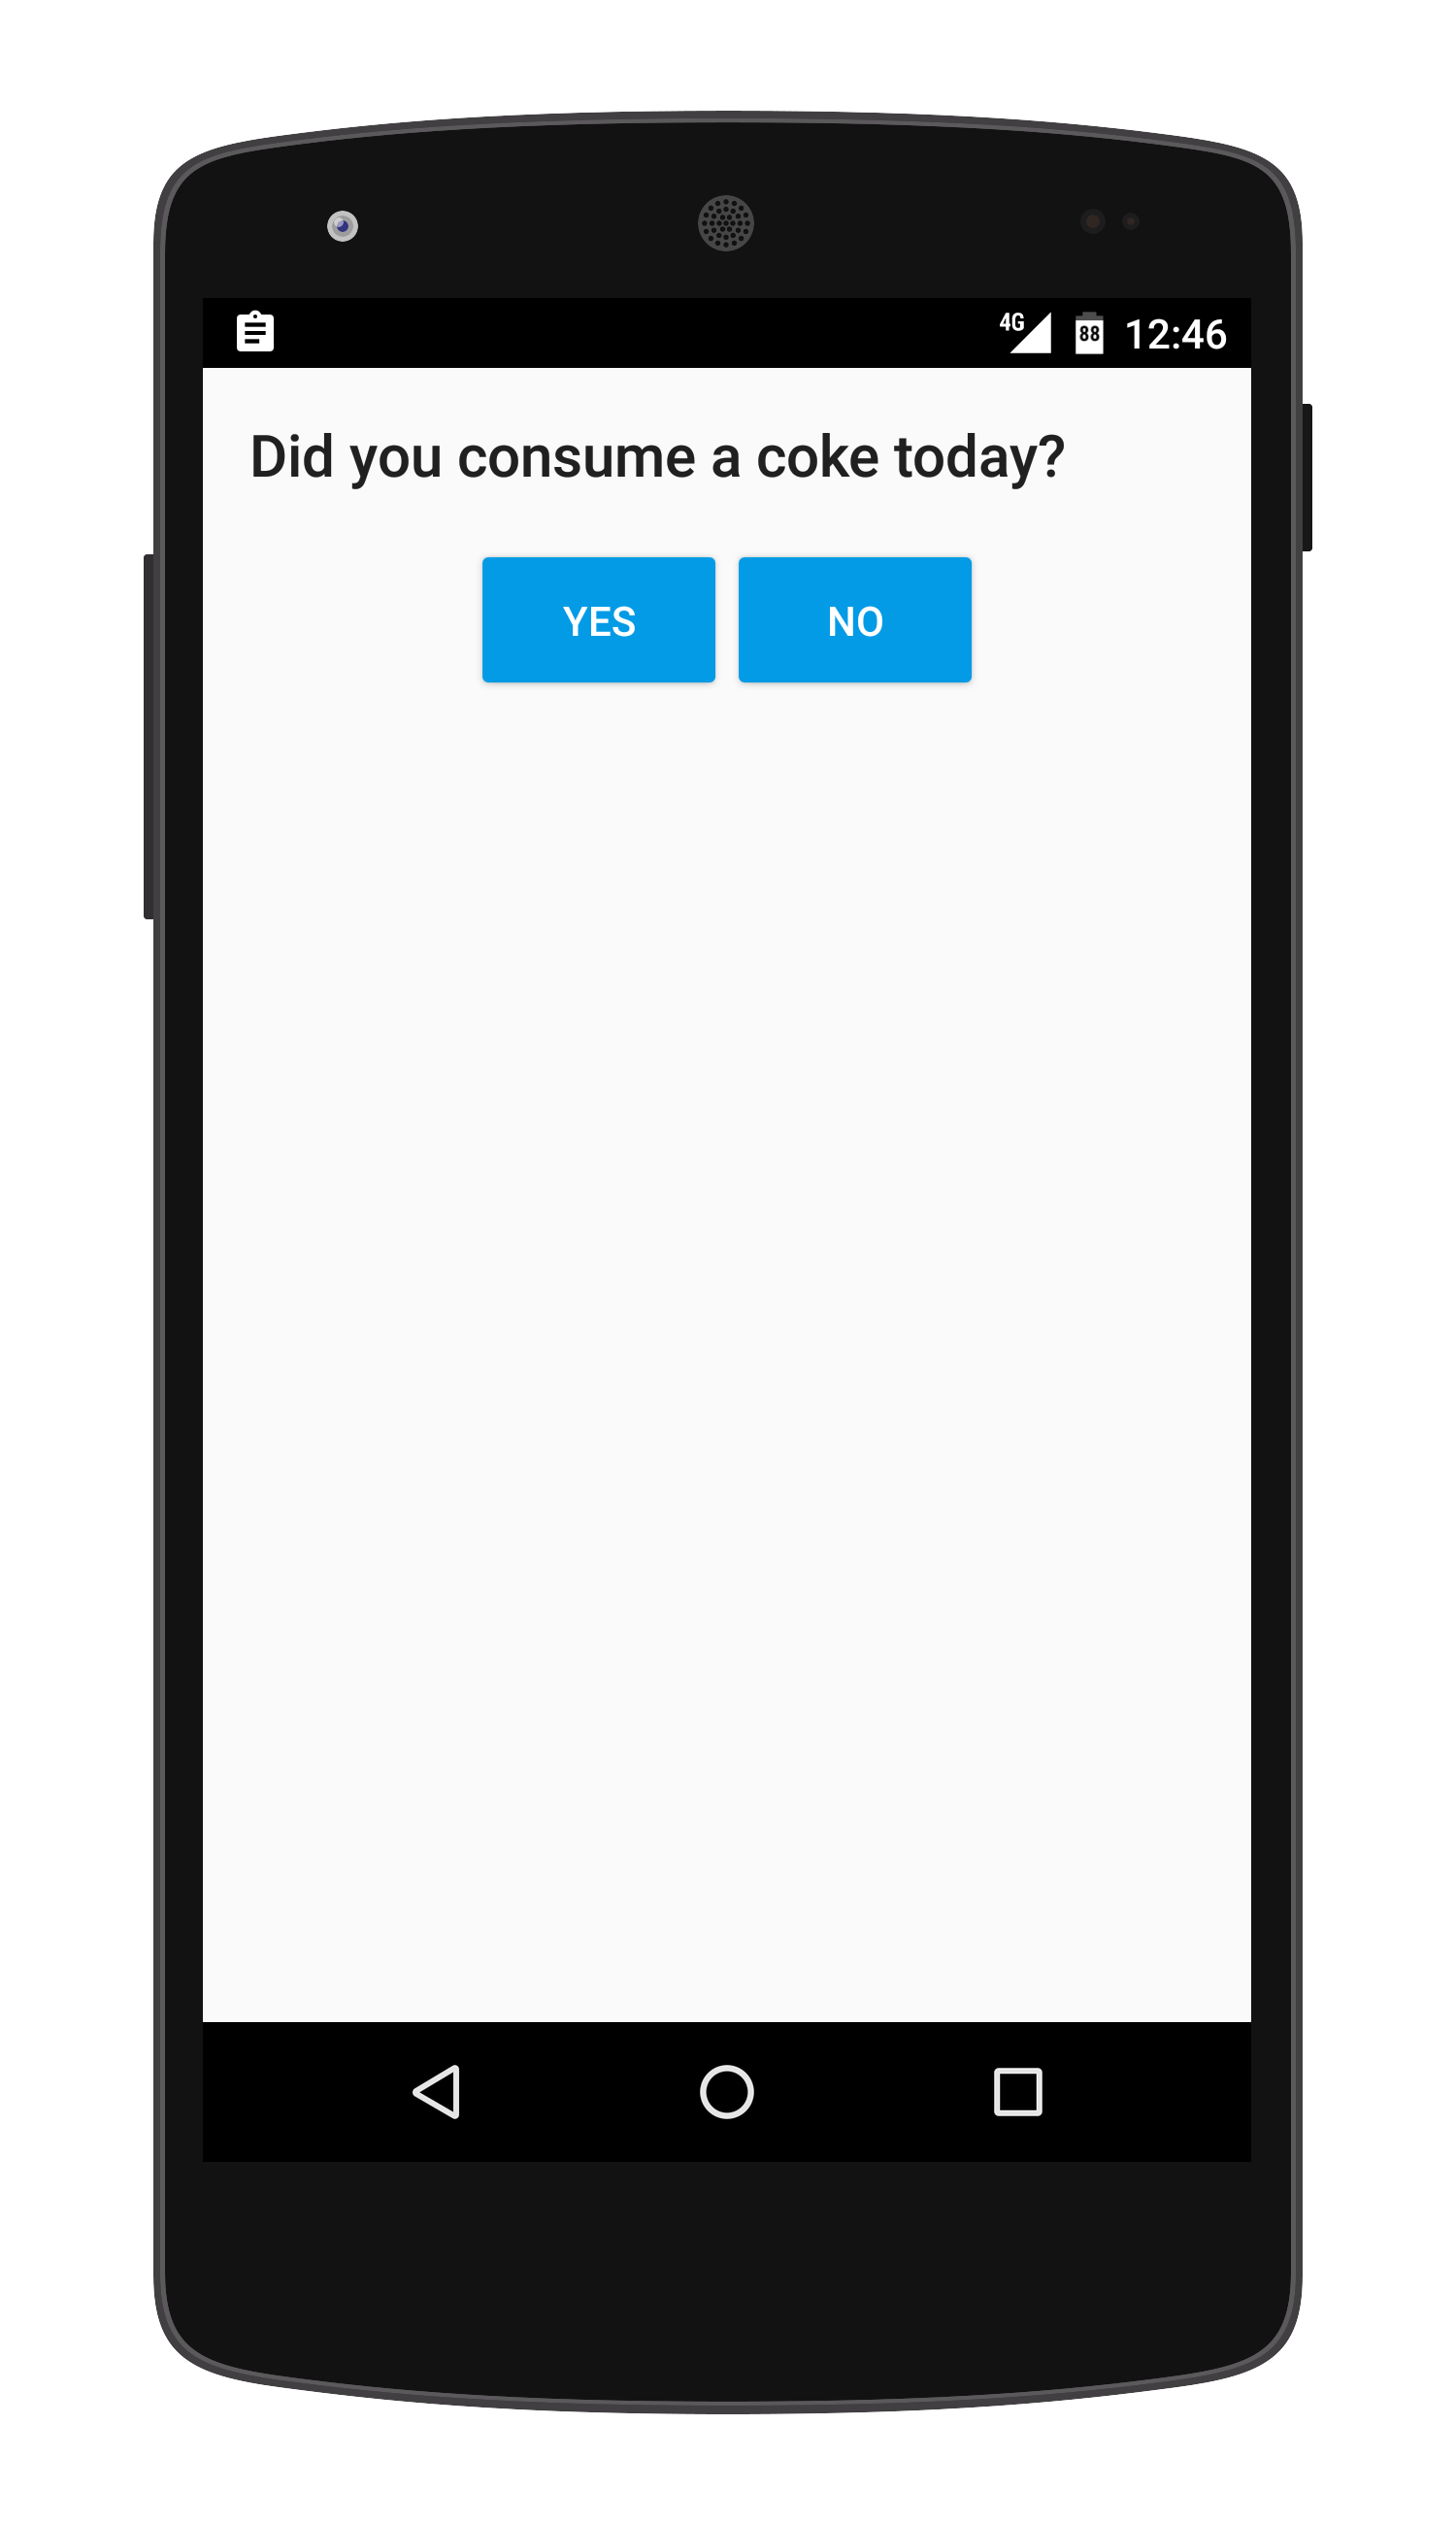
\includegraphics[width=.73\linewidth]{user_interfaces/client/client_answering_questions_with_phone}
        \caption{View when answering a question.}
        \label{fig:answering_questionnaire_answering}
    \end{subfigure}
    \caption{Questionnaire notification which is ready to be answered and view of a question being answered.}
    \label{fig:answering_questionnaire}
\end{figure}
\FloatBarrier

In the current implementation of the system, customers can only specify yes/no questions, but we have thought of different concepts for getting labels for snapshots:

\begin{description}
    \item[Complex questions] might be required for customers to get a better understanding of the label. Such questions could be: \emph{Which of the following statements would describe your current situation best?} or \emph{Please provide a small description of your current mood}. Questions such as the latter might be harder for customers to interpret automatically, but techniques such as sentiment analysis \parencite{pang2008opinion} could be applied here. The system should, ideally, not limit the customer in defining what label they would like to retrieve, i.e. customers should be able to define their own kind of question, or activity, they wish for participants to perform. 

    \item[Answer dependent questions] might be desired by customers to get a more detailed label, e.g. if the participants answers \emph{yes} to $q_1$, ask him $q_2$, otherwise ask $q_3$. Defining questions depending on the outcome of previous questions could become a complex task, and the customers might need visual aid in the creation of such questions.
    \\\\
    The customer interface might utilize some kind of drag and drop programming, like the programming platform for Lego Mindstorm\footnote{http://www.lego.com/da-dk/mindstorms/learn-to-program} to design questionnaires. With this the customer would be able to design the questionnaire just the way they want it, and be able to define exactly how they want to have their snapshots labeled. 
\end{description}

In the current application, questionnaires are triggered, and showed to the user, either in the start or the end of a snapshot, as described in \secref{sec:temporal_properties_of_snapshots}. This will cause the time of questionnaires to be relative to the time that the participants subscribed to the campaign. Some customers might instead be interested in questionnaires occurring at certain points of the day or occur when some event occur. Therefore we have considered some alternatives for triggering the questionnaires.

\begin{description}
    \item[Timely fixed triggers] might be useful to ensure that all participants are notified regarding questionnaires simultaneously, i.e. at a specific time of day. This might cause gathered information to be more easily related. Furthermore, customers might be interested in asking participants regarding something, only at a specific time, e.g. at eight in the morning. 

    \item[Event triggers] could be useful since participants is answering questions based on their own memory. So instead of waiting a fixed amount of time, triggers could be event based. This would prompt participants to answer questionnaires when a specific event occurs, e.g. when returning home, after finishing a call, or when a sensor reads a major fluctuation etc.    
\end{description}    